\chapter{Aplicaciones}\label{aplica}
\noindent Existen multitud de aplicaciones con ANNs, de forma más concreta, hay
aplicaciones para el reconocimiento de formas \cite{Roth2006}, aplicaciones clínicas
\cite{Dybowski2001} y en Biomedicina \cite{Lisboa2000}, aplicaciones en negocios
\cite{Lisboa2000b} y finanzas \cite{Kamruzzaman2006}, aplicaciones en teledetección
\cite{Gutierrez2009e,Gutierrez2007a}, etc. En
\cite{Bishop1995,Haykin2008,Murray2010,Rabunal2006} el lector puede estudiar más aplicaciones al
respecto, y en \cite{Paliwal2009} puede obtener una revisión muy reciente acerca de ello.

A continuación exponemos una aplicación en microbiología predictiva usando el algoritmo
MPENSGAII
desarrollado en esta tesis.

\section{Microbiología predictiva}
\noindent Hay muchos campos de estudio, como la medicina y la microbiología predictiva, donde
es muy importante predecir una variable de respuesta binaria, o equivalentemente, la
probabilidad de ocurrencia de un evento en términos de los valores de un conjunto de
variables explicativas relacionadas con ello \cite{Valero2007,Valero2007b,Garcia2009}.

Recientemente, debido a la demanda de productos alimenticios más saludables, se han
desarrollado varios modelos de clasificación en el campo de la microbiología predictiva
para evaluar
el comportamiento de microorganismos a partir de un conjunto dado de condiciones
\cite{Valero2009}
(envasado de ciertos productos lácteos, cárnicos, etc), ya que los científicos
reconocen que
existe una necesidad cada vez mayor para modelar los límites del crecimiento microbiano (fecha de
caducidad, fecha recomendada de consumo), como alternativa a las técnicas tradicionales en
microbiología, las cuales consumen mucho tiempo en la elaboración de experimentos
\cite{McMeekin1996,Ross2000}. Los modelos de crecimiento/no crecimiento cuantifican la probabilidad
de crecimiento microbiano, y definen las combinaciones de los factores de envasado
(temperatura (T), pH, actividad del agua (aW), etc) que impiden el mismo (el crecimiento
microbiano se
reduce a un número limitado de factores). Los modelos de predicción de crecimiento
microbiano se aceptan ampliamente como técnicas informativas que proporcionan
valoraciones rápidas y precisas sobre el mismo, y que se han
discutido por varios autores \cite{Schaffner1997,McMeekin2000}.

Dada una serie de patógenos, la respuesta de muchos de los microbios en los
alimentos se podría prever con conocimiento suficiente acerca de la formulación del
problema, de su tratamiento, y de las condiciones de almacenamiento de dichos alimentos para la
posterior elaboración de productos alimenticios, evitando el riesgo del crecimiento de un
determinado grupo de bacterias.

Los modelos de probabilidad de crecimiento de patógenos en los alimentos aparecieron en
la literatura en la década de 1970, cuando Genigeorgis \cite{Genigeorgis1971}, motivado
por la necesidad de predecir las combinaciones de las condiciones de envasado necesarias para evitar
el
crecimiento microbiano y la formación de toxinas, predijo el crecimiento a partir de un modelo de
reducción decimal de la bacteria \textit{Staphylococcus Aureus}. Un avance en este aspecto fue la
capacidad de predecir si un organismo crecería o no bajo un conjunto de condiciones
ambientales. Ratkowsky y Ross \cite{Ratkowsky1995} determinaron un modelo para predecir el
porcentaje de crecimiento bacteriano, incorporando el efecto de la temperatura, pH,
actividad de agua y la concentración de nitrito, a tal punto que podía predecir la
probabilidad de crecimiento.

\subsection{ANNs aplicadas a la microbiología predictiva}
\noindent Se han elaborado algunos trabajos de microbiología predictiva con ANNs
para modelar el crecimiento microbiano a lo largo del tiempo
\cite{Basheer2000,Schepers2000,Hajmeer2000}, así como para predecir los parámetros
de crecimiento, y de cómo el paso de dicho tiempo y el porcentaje de crecimiento
exponencial se ven
afectados por procesos bioquímicos extrínsecos y por condiciones ambientales
\cite{Jeyamkondan2001,Garcia2003,Garcia2005}.

De esta forma, Basheer y Hajmeer
\cite{Basheer2000} propusieron ANNs con activación hacia delante basándose en el criterio de
minimización del error mediante la retropropagación del mismo, aplicado al área de la
microbiología predictiva, junto con aplicaciones para la estimación de los parámetros de crecimiento
microbiano y la
modelización de la curva de crecimiento. Observaron experimentalmente que las ANNs
superaban a los enfoques más tradicionales de clasificación estadística.

En \cite{Schepers2000}, los autores  comparan ANNs con una sola capa oculta con métodos
estadísticos de reconocimiento de patrones
y otros aproximadores para encontrar el mejor modelo descriptivo de un conjunto de 20 curvas de
crecimiento del patógeno \textit{Lactobacillus helveticus}, con la obtención de buenos
resultados para los métodos con ANNs.

En \cite{Hajmeer2000}, Hajmeer y sus colaboradores
utilizan ANNs como aproximadores en funciones complejas de gran dimensionalidad, debido a
su alta no linealidad y a su tolerancia a los datos con ruido, de modo que los modelos
obtenidos se utilizaron para incluir el efecto del tiempo, así como una multitud de
parámetros relativos a las condiciones experimentales para los patógenos
\textit{Escherichia Coli 0157:H7} y \textit{Shigella Flexneri}.

En \cite{Jeyamkondan2001}
se comparan redes GRNN (\textit{General Regression Neural Networks}) con otros modelos
estadísticos, usando seis índices estadísticos y obteniendo buenos resultados en
generalización para las curvas de crecimiento de tres patógenos.

En \cite{Garcia2003,Garcia2005} García-Gimeno y colaboradores usan
modelos de ANNs con SUs para la estimación de varios parámetros cinéticos de
de los patógenos \textit{Leuconostoc Mesenteroides} y \textit{Escherichia Coli}, en
condiciones aeróbicas y anaeróbicas, comparando los resultados con un modelo de superficie
de respuesta, obteniendo modelos de predicción muy simples.

En \cite{Lou2001}, se
utilizan modelos de ANNs, y de nuevo se comparan con otras metodologías para predecir la
inactivación térmica de la bacteria \textit{Escherichia Coli}, obteniendo los mejores
resultados en precisión, gracias a la capacidad de las ANNs para calcular los efectos
combinados de los factores ambientales.

En \cite{Hajmeer2002}, se utilizan ANNs probabilísticas (\textit{Probabilistic
Neural Networks}), utilizando la estadística Bayesiana con el método de ventana de Parzen, de modo
que
se estimen las funciones de densidad de variables aleatorias en
la clasificación del crecimiento/no crecimiento del patógeno \textit{Escherichi Coli R31}, en
respuesta a la temperatura y actividad de agua.

En \cite{ElSebakhy2007,ElSebakhy2007b}, se utiliza un clasificador SVM (Support
Vector Machine) basado en funciones gaussianas  y un clasificador
neuro-difuso con funciones de pertenencia con forma de campana de Gauss, usando ANNs hacia delante
para la clasificación de los límites de crecimiento de \textit{Escherichi Coli R31}. Este mismo
patógeno se estudió en \cite{Hajmeer2003}, con clasificadores neuronales entrenados mediante el
método de retropropagación del error junto con ANNs probabilísticas (PNN), comparándose con
respecto a su precisión en la clasificación del crecimiento/no crecimiento, a partir de la
temperatura del agua, $T$, y de determinados valores de actividad de la misma, $aW$.

Recientemente, en \cite{Valero2007b}, se ha propuesto un nuevo enfoque para determinar la
probabilidad de crecimiento del patógeno \textit{Listeria Monocytogenes}, donde se aplica regresión
logística sobre una combinación de funciones lineales y transformaciones no lineales
de las mismas, donde las funciones lineales están formadas por las variables de
entrada, y las transformaciones son entrenadas por un AE con PUs, llamado EPUNN
(\textit{Evolutionary Product Unit Neural Network}).

Como se puede ver, se han hecho diversos trabajos con ANNs para resolver tareas
de clasificación en microbiología predictiva, pero en ningún caso, excepto en
\cite{Fernandez2008}, donde se usa un MOEA híbrido con ANNs de unidades SUs, se utiliza la
$MS$ para
mejorar la bondad de un clasificador en un marco multi-objetivo (ver
secciones \ref{ms-c} y \ref{propiedades} del capítulo
\ref{medidasRendimiento} y sección \ref{objetivosRedes} del capítulo \ref{MOEANNs}).

A continuación exponemos
la aplicación de nuestra metodología para la obtención de modelos de ANNs con funciones
de transferencia sigmoides, motivada por la demanda de los científicos sobre la necesidad de
modelar los límites el crecimiento microbiano de productos alimenticios más saludables.

\section{MPENSGAII en microbiología predictiva}
\noindent En esta sección presentamos la aplicación del algoritmo MPENSGAII en
microbiología predictiva \cite{Fernandez2009c} con el fin de obtener modelos de red que determinen
el crecimiento/no crecimiento de patógenos. Para ello, hemos utilizado
las mismas funciones objetivo para guiar el algoritmo que las descritas en la sección
\ref{funcionesObjetivo} del capítulo \ref{MOEANNs}, es decir, $E$ y
$MS$, los mismos operadores, el mismo algoritmo de LS, y las mismas etapas que utiliza
MPENSGAII. En esta ocasión hemos aplicado MPENSGAII a 4 patógenos en
microbiología predictiva.

\subsection{Diseño experimental}\label{disenioExperimental}
\noindent La regla de decisión que se utiliza con MPENSGAII para elegir automáticamente los modelos
del primer frente de Pareto es la de coger el mejor modelo en $E$,
y el mejor modelo en $MS$, (extremos del frente de Pareto), a partir de los
cuales calculamos la media y la desviación típica de $C$ y $MS$ en el conjunto de generalización,
para las 30 ejecuciones del algoritmo para cada conjunto de datos.

La manera de obtener el conjunto de entrenamiento y de generalización de los 4 conjuntos
de patógenos que hemos estudiado, no sigue el mismo procedimiento de partición
\textit{hold-out} que se hace en MPENSGAII, ya que los patrones de
los patógenos de los que disponemos se consiguen a partir de una experimentación previa por un
equipo de científicos especializados en microbiología predictiva (grupos de la Junta de
Andalucía, grupo de investigación AGR-170 HIBRO de el Plan Andaluz de Investigación,
Desarrollo e Innovación (PAIDI), director Gonzalo Zurera Cosano). Normalmente se hace
un
diseño factorial fraccional en forma de matriz, de manera que al hacer un
\textit{hol-out} estratificado podríamos perder todos los patrones de una determinada clase
para el conjunto de entrenamiento o para el conjunto de generalización (ver tabla
\ref{tabla9aplica} y la sección \ref{problemas}).

Los parámetros utilizados para los operadores de mutación (ver sección
\ref{operadoresMPENSGAII} del capítulo \ref{MOEANNs}), la asignación de pesos en la
creación de la población inicial (ver sección \ref{etapas} del capítulo \ref{MOEANNs}), el
tamaño de población, y los parámetros del algoritmo de LS iRprop+, son los mismos que los usados en
MPENSGAII (ver sección \ref{disenio} del capítulo \ref{MOEANNs}).

Para iniciar el procesamiento de datos de cada uno de los patógenos a clasificar, cada una
de las variables de entrada se escalaron en el intervalo $[-1.0, 1.0]$, para evitar así la
saturación de la señal.

Con el fin de comparar los resultados de nuestro algoritmo con algunos métodos
de referencia, usamos cuatro medidas de rendimiento: número de patrones correctamente
clasificados $C$, área bajo la curva ROC o $AUC$ (\textit{Area under Curve}), la mínima
sensibilidad, $MS$, y la raíz del error cuadrático medio o RMSE (\textit{Root Mean Square
Error}).
$C$, $AUC$, y $RMSE$ representan tres de las métricas más utilizadas en clasificación,
representando una
métrica de umbral, una métrica de probabilidad, y una métrica de rango respectivamente.
El lector puede obtener una información detallada de estas medidas en
\cite{Fawcett2006,Caruana2004}, o consultando el capítulo \ref{medidasRendimiento} de
este trabajo de tesis.

\subsection{Problemas seleccionados para testar MPENSGAII}\label{problemas}
\noindent Los 4 problemas de límite de crecimiento microbiano son de gran
importancia en la industria alimentaria, concretamente son los patógenos \textit{Listeria
Monocytogenes}, \textit{Escherichia Coli R31},
\textit{Staphylococcus
Aureus} y \textit{Shiguella Flexneri}.

\begin{description}
	\item[\textit{Listeria Monocytogenes}:] \textit{L. Monocytogenes} es un patógeno que proporciona
un grave problema relativo a las industrias de alimentos, debido a su ubicuidad en el
medio
natural
\cite{Hwang2005} y a las condiciones específicas de crecimiento del patógeno, que conducen
a su elevada prevalencia en diferentes tipos de productos alimenticios. Un impulso para
su investigación ha sido el problema de la listeriosis, y se han
propuesto diferentes estrategias para limitar los niveles de contaminación en el momento
del consumo a menos de 100 UFC/g (Comisión Europea \cite{Commission1999}).

Los datos de \textit{L. Monocytogenes} se recogieron previamente por un grupo de especialistas en
microbiología predictiva para encontrar sus límites de crecimiento, con concentraciones de CA (ácido
cítrico) y AA (ácido ascórbico) de $0$, $0\text{\textquotestraightbase}05$,
$0\text{\textquotestraightbase}1$, $0\text{\textquotestraightbase}15$,
$0\text{\textquotestraightbase}2$,
$0\text{\textquotestraightbase}25$, $0\text{\textquotestraightbase}3$,
$0\text{\textquotestraightbase}35$ y $0\text{\textquotestraightbase}4$\%
$(w/v)$ (water/volume, es decir, 0\text{\textquotestraightbase}4 significa
0\text{\textquotestraightbase}4
mL de ácido en 100 mL del medio), a $4$, $7$, $10$, $15$ y $30$ \textcelsius,
y niveles de pH de $4\text{\textquotestraightbase}5$, $5$, $5\text{\textquotestraightbase}5$ y $6$,
como se puede
ver en \cite{Valero2007b}. Así,  se probaron 39 condiciones diferentes, con ocho replicas por
condición. El conjunto de datos del patógeno se divide de manera que, 404  condiciones
se usaron para
entrenamiento, y 135 para generalización. De las 539 diferentes posibles curvas de
crecimiento, hubo 299 de crecimiento y 240 de no crecimiento.

Para determinar los datos pertenecientes al conjunto de entrenamiento y al conjunto de
generalización, se han seleccionado alternativamente las condiciones de los ácidos orgánicos
utilizados en el mismo nivel de temperatura y pH, como se muestra en la tabla \ref{tabla9aplica}. El
objetivo de esta selección fue definir los datos del conjunto de entrenamiento que realmente
representan
las zonas limítrofes, con el fin de obtener un mejor ajuste. La cantidad de ácidos añadidos
se calculó en porcentaje (w/v), con el fin de imitar la adición de ácidos orgánicos que tiene lugar
en las industrias de alimentos. Exámenes previos revelan que el uso de la concentración de ácido no
disociado (UAC) como un factor independiente da lugar a modelos más precisos que cuando se usa
la concentración total de ácidos. Esta es una observación razonable, ya que ha quedado
claramente demostrado que UAC de ácidos orgánicos es la molécula efectiva que causa la inhibición
del crecimiento \cite{ICMSF1980}.

\begin{table}[!htb]
\caption{Diseño experimental seguido en un mismo nivel de temperatura y de pH.}
\label{tabla9aplica}
\centering
\tabcolsep 6pt
\begin{tabular}{cccccccccc} \hline
\rowcolor[rgb]{0.70,0.85,1} CA(\%) & \textbf{0} &\textbf{ 0.05} & \textbf{0.1} & \textbf{0.15} &
\textbf{0.2} & \textbf{0.25} & \textbf{0.3} &\textbf{0.35} &\textbf{0.4} \\
\rowcolor[rgb]{0.70,0.85,1} AA(\%) &  & & & & & & & & \\ \hline
\rowcolor[rgb]{0.86,0.94,1} \cellcolor[rgb]{0.70,0.85,1} \textbf{0} & \textopenbullet &
$\blacklozenge$ & \textopenbullet & $\blacklozenge$ & \textopenbullet & $\blacklozenge$ &
\textopenbullet & $\blacklozenge$ & \textopenbullet \\
\rowcolor[rgb]{0.86,0.94,1} \cellcolor[rgb]{0.70,0.85,1} \textbf{0.05} & $\blacklozenge$ &
\textopenbullet &
$\blacklozenge$ & \textopenbullet & $\blacklozenge$ & \textopenbullet & $\blacklozenge$ &
\textopenbullet & $\blacklozenge$ \\
\rowcolor[rgb]{0.86,0.94,1} \cellcolor[rgb]{0.70,0.85,1} \textbf{0.1} &  \textopenbullet &
$\blacklozenge$ &
\textopenbullet & $\blacklozenge$ & \textopenbullet & $\blacklozenge$ & \textopenbullet
& $\blacklozenge$ & \textopenbullet \\
\rowcolor[rgb]{0.86,0.94,1} \cellcolor[rgb]{0.70,0.85,1} \textbf{0.15} & $\blacklozenge$ &
\textopenbullet &
$\blacklozenge$ & \textopenbullet & $\blacklozenge$ & \textopenbullet & $\blacklozenge$ &
\textopenbullet & $\blacklozenge$ \\
\rowcolor[rgb]{0.86,0.94,1} \cellcolor[rgb]{0.70,0.85,1} \textbf{0.2} &  \textopenbullet &
$\blacklozenge$ &
\textopenbullet & $\blacklozenge$ & \textopenbullet & $\blacklozenge$ & \textopenbullet
& $\blacklozenge$ & \textopenbullet \\
\rowcolor[rgb]{0.86,0.94,1} \cellcolor[rgb]{0.70,0.85,1} \textbf{0.25} & $\blacklozenge$ &
\textopenbullet &
$\blacklozenge$ & \textopenbullet & $\blacklozenge$ & \textopenbullet & $\blacklozenge$ &
\textopenbullet & $\blacklozenge$ \\
\rowcolor[rgb]{0.86,0.94,1} \cellcolor[rgb]{0.70,0.85,1} \textbf{0.3} &  \textopenbullet &
$\blacklozenge$ &
\textopenbullet & $\blacklozenge$ & \textopenbullet & $\blacklozenge$ & \textopenbullet
& $\blacklozenge$ & \textopenbullet \\
\rowcolor[rgb]{0.86,0.94,1} \cellcolor[rgb]{0.70,0.85,1} \textbf{0.35} & $\blacklozenge$ &
\textopenbullet &
$\blacklozenge$ & \textopenbullet & $\blacklozenge$ & \textopenbullet & $\blacklozenge$ &
\textopenbullet & $\blacklozenge$ \\
\rowcolor[rgb]{0.86,0.94,1} \cellcolor[rgb]{0.70,0.85,1} \textbf{0.4} &  \textopenbullet &
$\blacklozenge$ &
\textopenbullet & $\blacklozenge$ & \textopenbullet & $\blacklozenge$ & \textopenbullet
& $\blacklozenge$ & \textopenbullet \\ \hline
\multicolumn{10}{l}{CA = Ácido citrico, AA = Ácido ascórbico.} \\
\multicolumn{10}{l}{\textopenbullet = patrones de entrenamiento, $\blacklozenge$ = patrones
de generalización.}
\end{tabular}
\end{table}

\item[\textit{Escherichia Coli R31}:] Este
patógeno lo proporcionó Salter y colaboradores en \cite{Salter2000}, y pertenece al crecimiento/ no
crecimiento de una cepa de \textit{Escherichia Coli}, concretamente la cepa \textit{R31}, la cual se
ve afectada por la temperatura y actividad del agua.

Los datos obtenidos provienen de experimentos realizados con diferentes combinaciones de
temperatura en el intervalo $7\text{\textquotestraightbase}7-37\text{\textquotestraightbase}0$, y la
actividad de agua en el intervalo
$0\text{\textquotestraightbase}943-0\text{\textquotestraightbase}987$. Todas las muestras de
\textit{E. Coli R31} se cultivaron en placas y
tubos-L observados diariamente. Si se produce crecimiento en una muestra, se considera
como resultado positivo. El crecimiento en las muestras se observa por un visible
aumento de la turbidez o por depósitos en el tubo-L. Si después de 50 días no hay
turbidez o depósitos, se extiende un asa de cultivos sobre placas incluyendo agar,
para determinar si estuvo presente algún crecimiento. Se observaron un total de
179 muestras utilizando diferentes valores de temperatura y actividad del
agua, con 99 casos de decrecimiento y el 80 de no crecimiento.

\item[\textit{Staphylococcus Aureus}:] El patógeno \textit{S. Aureus} se ha
reconocido como un indicador de la deficiencia de higiene en los alimentos y una causa
importante de gastroenteritis en todo el mundo \cite{Soriano2002}. Para conocer los
límites de crecimiento de S. Aureus \cite{Valero2009} se utilizó un diseño factorial
fraccional. Cuidadosamente se eligió un subconjunto (fracción) de los experimentos de un diseño
factorial completo con el fin de reducir el tiempo de experimentación y los recursos. La selección
se basó en la delimitación de los niveles de los factores ambientales estudiados para el
dominio de crecimiento/no crecimiento de \textit{S. Aureus}. Dado que no se ha
detectado un crecimiento de $7\text{\textquotestraightbase}5$ \textcelsius, o por debajo, los datos
se recopilaron a
$8$, $10$, $13$, $16$ y $19$ \textcelsius, y a niveles de pH de $4\text{\textquotestraightbase}5$ a
$7\text{\textquotestraightbase}5$ (en
intervalos de $0\text{\textquotestraightbase}5$) y en 19 niveles actividad del agua (aW) (desde
$0\text{\textquotestraightbase}856$ a $0\text{\textquotestraightbase}999$ a intervalos regulares).

El patógeno inicial (287 condiciones) se dividió en dos partes: un conjunto de
entrenamiento con 146 condiciones, cubriendo los extremos, y un conjunto de generalización,
con 141 condiciones, dentro de la región de interpolación del modelo. Para las diferentes
condiciones de los factores ambientales, se produjeron 162 casos de crecimiento y 125 de no
crecimiento. El objetivo
de esta selección fue definir un patógeno  centrado en
las regiones extremas del dominio de crecimiento/no crecimiento, que representan
las zonas fronterizas. En este estudio, el número de réplicas por condición $(n=30)$ se
incrementó en comparación con otros estudios, para obtener el punto de transición de
crecimiento/no crecimiento.

\item[\textit{Shiguella Flexneri}:] \textit{S. Flexneri} es un importante agente
	causante de enfermedades gastrointestinales \cite{Zaika1994}. Para evaluar los
efectos de la temperatura se utilizó un diseño factorial incompleto con valores de $12$,
$15$, $19$, $28$, $37$ \textcelsius, un pH inicial de $5\text{\textquotestraightbase}5$,
$6\text{\textquotestraightbase}0$, $6\text{\textquotestraightbase}5$,
$7\text{\textquotestraightbase}0$, $7\text{\textquotestraightbase}5$,
cloruro de sodio con valores de $0\text{\textquotestraightbase}5$, $2\text{\textquotestraightbase}5$
y $4\text{\textquotestraightbase}0$\%, y nitrito de sodio con valores de
$0$, $50$, $100$, $200$ y $1000$ ppm. Los datos se obtuvieron a partir de 375 cultivos, lo
que supone 123 combinaciones de variables. El número de réplicas de cultivos probados para
cada combinación de variables se da en la Tabla 2 del artículo \cite{Zaika1994}. Estos datos se
utilizaron para obtener los modelos y predecir el
crecimiento anaeróbico de \textit{S. Flexneri} en función de la temperatura, las
concentraciones de cloruro de sodio, nitrito de sodio y el pH inicial.

La cinética de crecimiento de los datos para cada combinación de variables se resumen en
la tabla 2 del artículo al que se ha hecho referencia. El crecimiento de \textit{S.
Flexneri} no
se observó bajo las condiciones correspondientes a 40 de las combinaciones de variables
estudiadas. Se estudiaron 15 combinaciones adicionales de variables originadas en entornos
ambientales, donde algunas de las replicas del cultivo crecieron, mientras que
otras no lo hicieron (detallado en la Tabla 3 del artículo citado).
\end{description}

En la tabla \ref{tabla1aplica} podemos ver las características de cada
patógeno. Se muestra el número total de patrones, el
número de patrones en los conjuntos de entrenamiento y generalización, el número de
variables de entrada, el número total de patrones por clase y el valor de $p^*$ (el
mínimo de las probabilidades estimadas ``a priori``). Para cada conjunto de datos se ha
utilizado un diseño factorial fraccional, con el fin de
averiguar los límites de crecimiento de cada microorganismo.

\begin{table}[!htb]
\scriptsize
\caption{Características de los patógenos \textit{Listeria Monocytogenes},
\textit{Escherichia Coli R31}, \textit{Staphylococcus Aureus} y \textit{Shigella
Flexneri}.}
\label{tabla1aplica}
\centering
\tabcolsep 4pt
\begin{tabular}{lcccc} \hline
\rowcolor[rgb]{0.70,0.85,1} & \textbf{L. Monocytogenes} &
\textbf{E. Coli R31} & \textbf{S. Aureus} & \textbf{S. Flexneri} \\ \hline
\rowcolor[rgb]{0.86,0.94,1} \textbf{Patrones} & 539 & 179 & 287 & 123 \\
\rowcolor[rgb]{0.86,0.94,1} \textbf{Patrones entrenamiento} & 404 & 134 & 146 & 76 \\
\rowcolor[rgb]{0.86,0.94,1}  \textbf{Patrones generalización} & 135 & 45 & 141 & 47 \\
\rowcolor[rgb]{0.86,0.94,1} \textbf{Variables de entrada} & 4 & 2 & 3 & 4 \\
\rowcolor[rgb]{0.86,0.94,1} \textbf{Patrones por clase} & 299-240 & 99-80 & 162-125 &
79-44 \\
\rowcolor[rgb]{0.86,0.94,1} \textbf{p*} & 0.44 & 0.44 & 0.43 & 0.32 \\ \hline
\multicolumn{4}{l}{La primera clase significa crecimiento, la segunda no crecimiento.}
\end{tabular}
\end{table}

\subsection{Resultados}
\noindent Las métricas que hemos mencionado en la sección \ref{disenioExperimental} las
hemos utilizado para comparar el rendimiento de MPENSGAII con 11 algoritmos bien conocidos
y usados en \textit{Machine Learning}: Adaboost M1, BayesNet, C4.5, KStar, LivSVM,
Logistic Model Tree, MultiLogistic, NaivesBayesUpdateable, NBTree, SimpleLogistic y
RandomForest. Para consultar la descripción de cada uno de estos 11 algoritmos y de sus parámetros
el lector se puede referir a \cite{Landwehr2005}, y también están disponibles en WEKA
\footnote{http://www.cs.waikato.ac.nz/ml/weka/} \cite{Witten2005}, aplicación que hemos
utilizado para los experimentos realizados con dichos algoritmos. LibSVM es un
paquete software que está disponible y actualizado continuamente para máquinas de soporte vectorial
(SVM) \footnote{http://www.csie.ntu.edu.tw/$\sim$cjlin/libsvm} \cite{Chang2001}.

Los valores de los parámetros para cada algoritmo y para cada patógeno se eligieron en
base a una batería de pruebas, seleccionando los parámetros que para cada patógeno dieron el mejor
resultado. La batería de pruebas realizada considera los valores que van desde el límite
inferior de cada parámetro, pasando por los valores intermedios y llegando hasta el valor del límite
superior de los mismos.

A continuación hacemos una breve descripción de los parámetros de los algoritmos con los
que hemos comparado, y de la nomenclatura seguida en cuanto al nombre de cada parámetro y
el nombre del algoritmo, para así poder entender las abreviaturas nemotécnicas de la tabla
\ref{tabla2aplica} (nos ha sido necesario abreviar sus nombres para poder prodecer a
una lectura más fácil de las tablas que se mostrarán más adelante).

\begin{table}[!htb]
\caption{Parámetros optimizados para los algoritmos Adaboost M1, BayesNet, C4.5 o J48,
LMT, MultiLogistic y SimpleLogistic. Para una completa descripción de cada parámetro
consultar estos algoritmos en WEKA.}
\label{tabla2aplica}
\scriptsize
\centering
\tabcolsep 7pt
\begin{tabular}{lcccccccc} \hline
\multicolumn{9}{>{\columncolor[rgb]{0.70,0.85,1}}c}{\textbf{AdaBoost M1}} \\ \hline
\rowcolor[rgb]{0.70,0.85,1}\textbf{Patógeno} &
\multicolumn{2}{>{\columncolor[rgb]{0.70,0.85,1}}c}{\textbf{BC}} &
\multicolumn{2}{>{\columncolor[rgb]{0.70,0.85,1}}c}{\textbf{IT}} &
\multicolumn{2}{>{\columncolor[rgb]{0.70,0.85,1}}c}{\textbf{RS}} &
\multicolumn{2}{>{\columncolor[rgb]{0.70,0.85,1}}c}{\textbf{WT}}  \\ \hline
\rowcolor[rgb]{0.86,0.94,1}\textbf{Listeria} &
\multicolumn{2}{>{\columncolor[rgb]{0.86,0.94,1}}c}{C4.5} &
\multicolumn{2}{>{\columncolor[rgb]{0.86,0.94,1}}c}{100} &
\multicolumn{2}{>{\columncolor[rgb]{0.86,0.94,1}}c}{False} &
\multicolumn{2}{>{\columncolor[rgb]{0.86,0.94,1}}c}{100}  \\
\rowcolor[rgb]{0.86,0.94,1}\textbf{E. Coli} &
\multicolumn{2}{>{\columncolor[rgb]{0.86,0.94,1}}c}{C4.5} &
\multicolumn{2}{>{\columncolor[rgb]{0.86,0.94,1}}c}{100} &
\multicolumn{2}{>{\columncolor[rgb]{0.86,0.94,1}}c}{False} &
\multicolumn{2}{>{\columncolor[rgb]{0.86,0.94,1}}c}{150} \\
\rowcolor[rgb]{0.86,0.94,1}\textbf{S. Aureus} &
\multicolumn{2}{>{\columncolor[rgb]{0.86,0.94,1}}c}{C4.5} &
\multicolumn{2}{>{\columncolor[rgb]{0.86,0.94,1}}c}{100} &
\multicolumn{2}{>{\columncolor[rgb]{0.86,0.94,1}}c}{False} &
\multicolumn{2}{>{\columncolor[rgb]{0.86,0.94,1}}c}{50}  \\
\rowcolor[rgb]{0.86,0.94,1}\textbf{S. Flexneri} &
\multicolumn{2}{>{\columncolor[rgb]{0.86,0.94,1}}c}{C4.5} &
\multicolumn{2}{>{\columncolor[rgb]{0.86,0.94,1}}c}{100} &
\multicolumn{2}{>{\columncolor[rgb]{0.86,0.94,1}}c}{False} &
\multicolumn{2}{>{\columncolor[rgb]{0.86,0.94,1}}c}{150} \\ \hline
\multicolumn{9}{>{\columncolor[rgb]{0.70,0.85,1}}c}{\textbf{BayesNet}} \\ \hline
\rowcolor[rgb]{0.70,0.85,1}\textbf{Patógeno} &
\multicolumn{5}{>{\columncolor[rgb]{0.70,0.85,1}}c}{\textbf{EA}} &
\multicolumn{3}{>{\columncolor[rgb]{0.70,0.85,1}}c}{\textbf{SA}} \\ \hline
\rowcolor[rgb]{0.86,0.94,1}\textbf{Listeria} &
\multicolumn{5}{>{\columncolor[rgb]{0.86,0.94,1}}c}{Simple Estimator} &
\multicolumn{3}{>{\columncolor[rgb]{0.86,0.94,1}}c}{Simulated Annealing} \\
\rowcolor[rgb]{0.86,0.94,1}\textbf{E. Coli} &
\multicolumn{5}{>{\columncolor[rgb]{0.86,0.94,1}}c}{Simple Estimator} &
\multicolumn{3}{>{\columncolor[rgb]{0.86,0.94,1}}c}{Simulated Annealing} \\
\rowcolor[rgb]{0.86,0.94,1}\textbf{S. Aureus} &
\multicolumn{5}{>{\columncolor[rgb]{0.86,0.94,1}}c}{BMA Estimator} &
\multicolumn{3}{>{\columncolor[rgb]{0.86,0.94,1}}c}{Tabu Search} \\
\rowcolor[rgb]{0.86,0.94,1}\textbf{S. Flexneri} &
\multicolumn{5}{>{\columncolor[rgb]{0.86,0.94,1}}c}{Simple Estimator} &
\multicolumn{3}{>{\columncolor[rgb]{0.86,0.94,1}}c}{Simulated Annealing} \\ \hline
\multicolumn{9}{>{\columncolor[rgb]{0.70,0.85,1}}c}{\textbf{C4.5 o J48}} \\ \hline
\rowcolor[rgb]{0.70,0.85,1}\textbf{Patógeno} &
\multicolumn{2}{>{\columncolor[rgb]{0.70,0.85,1}}c}{\textbf{CF}} &
\multicolumn{3}{>{\columncolor[rgb]{0.70,0.85,1}}c}{\textbf{NI}} &
\multicolumn{3}{>{\columncolor[rgb]{0.70,0.85,1}}c}{\textbf{AD}} \\ \hline
\rowcolor[rgb]{0.86,0.94,1}\textbf{Listeria} &
\multicolumn{2}{>{\columncolor[rgb]{0.86,0.94,1}}c}{0.1} &
\multicolumn{3}{>{\columncolor[rgb]{0.86,0.94,1}}c}{2} &
\multicolumn{3}{>{\columncolor[rgb]{0.86,0.94,1}}c}{2} \\
\rowcolor[rgb]{0.86,0.94,1}\textbf{E. Coli} &
\multicolumn{2}{>{\columncolor[rgb]{0.86,0.94,1}}c}{0.5} &
\multicolumn{3}{>{\columncolor[rgb]{0.86,0.94,1}}c}{5} &
\multicolumn{3}{>{\columncolor[rgb]{0.86,0.94,1}}c}{5} \\
\rowcolor[rgb]{0.86,0.94,1}\textbf{S. Aureus} &
\multicolumn{2}{>{\columncolor[rgb]{0.86,0.94,1}}c}{0.25} &
\multicolumn{3}{>{\columncolor[rgb]{0.86,0.94,1}}c}{3} &
\multicolumn{3}{>{\columncolor[rgb]{0.86,0.94,1}}c}{3} \\
\rowcolor[rgb]{0.86,0.94,1}\textbf{S. Flexneri} &
\multicolumn{2}{>{\columncolor[rgb]{0.86,0.94,1}}c}{0.1} &
\multicolumn{3}{>{\columncolor[rgb]{0.86,0.94,1}}c}{2} &
\multicolumn{3}{>{\columncolor[rgb]{0.86,0.94,1}}c}{2} \\ \hline
\multicolumn{9}{>{\columncolor[rgb]{0.70,0.85,1}}c}{\textbf{LMT}} \\ \hline
\rowcolor[rgb]{0.70,0.85,1}\textbf{Patógeno} &
\multicolumn{2}{>{\columncolor[rgb]{0.70,0.85,1}}c}{\textbf{MI}} &
\multicolumn{3}{>{\columncolor[rgb]{0.70,0.85,1}}c}{\textbf{LB}} &
\multicolumn{3}{>{\columncolor[rgb]{0.70,0.85,1}}c}{\textbf{BV}} \\ \hline
\rowcolor[rgb]{0.86,0.94,1}\textbf{Listeria} &
\multicolumn{2}{>{\columncolor[rgb]{0.86,0.94,1}}c}{15} &
\multicolumn{3}{>{\columncolor[rgb]{0.86,0.94,1}}c}{10} &
\multicolumn{3}{>{\columncolor[rgb]{0.86,0.94,1}}c}{0.1} \\
\rowcolor[rgb]{0.86,0.94,1}\textbf{E. Coli} &
\multicolumn{2}{>{\columncolor[rgb]{0.86,0.94,1}}c}{5} &
\multicolumn{3}{>{\columncolor[rgb]{0.86,0.94,1}}c}{-1} &
\multicolumn{3}{>{\columncolor[rgb]{0.86,0.94,1}}c}{0.0} \\
\rowcolor[rgb]{0.86,0.94,1}\textbf{S. Aureus} &
\multicolumn{2}{>{\columncolor[rgb]{0.86,0.94,1}}c}{15} &
\multicolumn{3}{>{\columncolor[rgb]{0.86,0.94,1}}c}{10} &
\multicolumn{3}{>{\columncolor[rgb]{0.86,0.94,1}}c}{0.1} \\
\rowcolor[rgb]{0.86,0.94,1}\textbf{S. Flexneri} &
\multicolumn{2}{>{\columncolor[rgb]{0.86,0.94,1}}c}{25} &
\multicolumn{3}{>{\columncolor[rgb]{0.86,0.94,1}}c}{20} &
\multicolumn{3}{>{\columncolor[rgb]{0.86,0.94,1}}c}{0.2} \\ \hline
\multicolumn{9}{>{\columncolor[rgb]{0.70,0.85,1}}c}{\textbf{MultiLogistic}} \\ \hline
\rowcolor[rgb]{0.70,0.85,1}\textbf{Patógeno} &
\multicolumn{4}{>{\columncolor[rgb]{0.70,0.85,1}}c}{\textbf{IT}} &
\multicolumn{4}{>{\columncolor[rgb]{0.70,0.85,1}}c}{\textbf{RL}} \\ \hline
\rowcolor[rgb]{0.86,0.94,1}\textbf{Listeria} &
\multicolumn{4}{>{\columncolor[rgb]{0.86,0.94,1}}c}{5} &
\multicolumn{4}{>{\columncolor[rgb]{0.86,0.94,1}}c}{10-8} \\
\rowcolor[rgb]{0.86,0.94,1}\textbf{E. Coli} &
\multicolumn{4}{>{\columncolor[rgb]{0.86,0.94,1}}c}{5} &
\multicolumn{4}{>{\columncolor[rgb]{0.86,0.94,1}}c}{10-8} \\
\rowcolor[rgb]{0.86,0.94,1}\textbf{S. Aureus} &
\multicolumn{4}{>{\columncolor[rgb]{0.86,0.94,1}}c}{5} &
\multicolumn{4}{>{\columncolor[rgb]{0.86,0.94,1}}c}{10-8} \\
\rowcolor[rgb]{0.86,0.94,1}\textbf{S. Flexneri} &
\multicolumn{4}{>{\columncolor[rgb]{0.86,0.94,1}}c}{5} &
\multicolumn{4}{>{\columncolor[rgb]{0.86,0.94,1}}c}{10-8}\\ \hline
\multicolumn{9}{>{\columncolor[rgb]{0.70,0.85,1}}c}{\textbf{SimpleLogistic}} \\ \hline
\rowcolor[rgb]{0.70,0.85,1}\textbf{Patógeno} & \textbf{ER} & \textbf{HS} & \textbf{MI} &
\multicolumn{2}{>{\columncolor[rgb]{0.70,0.85,1}}c}{\textbf{NI}} & \textbf{AIC} &
\textbf{CV} & \textbf{BV} \\ \hline
\rowcolor[rgb]{0.86,0.94,1}\textbf{Listeria} & False & 100 & 900 &
\multicolumn{2}{>{\columncolor[rgb]{0.86,0.94,1}}c}{10}
& False & True & 0.0 \\
\rowcolor[rgb]{0.86,0.94,1}\textbf{E. Coli} & False & 100 & 900 &
\multicolumn{2}{>{\columncolor[rgb]{0.86,0.94,1}}c}{10} &
False & True & 0.0 \\
\rowcolor[rgb]{0.86,0.94,1}\textbf{S. Aureus} & False & 100 & 900 &
\multicolumn{2}{>{\columncolor[rgb]{0.86,0.94,1}}c}{10}
& False & True & 0.0 \\
\rowcolor[rgb]{0.86,0.94,1}\textbf{S. Flexneri} & False & -1 & 900 &
\multicolumn{2}{>{\columncolor[rgb]{0.86,0.94,1}}c}{-10} & False & True & 0.0 \\ \hline
\end{tabular}
\end{table}

Los paramétros de los algoritmos utilizados en la tabla \ref{tabla2aplica} y la nomenclatura
seguida para los mismos, se nombran a continuación:

\begin{description}
	\item[AdaBoost M1 (AB):] Clasificador base (BC), número de iteraciones (IT), uso de
remuestreo (RS) y umbral de pesos para la poda (WT).
   \item[BayesNet (BN):] Algoritmo de estimación (EA) y algoritmo para la búsqueda de la
estructura de las redes (SA).
   \item[C4.5 o J48:] Factor de confianza para la poda (CF), número mínimo de instancias
por hoja (NI) y cantidad de datos para reducir el error de poda (AD).
   \item[KStar (KS):] Mezcla global (GB). Este parámetro es el único que se utiliza con
KStar en WEKA. Todos los experimentos han utilizado un valor de 20, excepto para \textit{S.
Flexneri}, que utiliza un valor de 50.
   \item[LibSVM (LSVM):] La librería software LibSVM para máquinas de soporte vectorial
(SVM), contiene una secuencia de mandatos para ajustar automáticamente los
hiper-parámetros asociados a este tipo de modelos, incluyendo el parámetro de coste y el
ancho de los centros Gaussianos. La biblioteca busca los mejores valores de los hiper-parámetros
mediante una búsqueda matricial o en \textit{grid} y escoge la mejor configuración
mediante un proceso de validación cruzada \textit{10-fold-crossvalidation}
\cite{Chang2001}.
   \item[Logistic Model Tree (LMT):] Número mínimo de instancias o patrones que se pueden
considerar para dividir un nodo (MI), número de iteraciones para LogitBoost (LB) y el
porcentaje de recorte de pesos en LogitBoost (BV).
   \item[MultiLogistic o Logistic (ML):] Máximo número de iteraciones (IT) y valor de
verosimilitud (RL).
   \item[NaivesBayesUpdateable (NB):] Estimador de \textit{kernel} para
    atributos numéricos en lugar de una distribución normal (KS). En este caso KS se
	seleccionó para todos los experimentos (proporcionaba mejores resultados).
	   \item[NBTree (NBT):] WEKA solo proporciona una configuración por defecto para este
algoritmo, que es la que se ha utilizado para todos los experimentos.
   \item[SimpleLogistic (SL):] Error en las probabilidades (ER), parada heurística (HS),
máximo número de iteraciones para LogitBoost (MI), número de iteraciones para LogitBoost
(NI), AIC para determinar cuando parar las iteraciones de LogitBoost (AIC), validación
cruzada para LogitBoost (CV) y porcentaje de recorte de pesos en LogitBoost (BV).
\item[RandomForest (RF):] Profundidad máxima de los árboles, número de atributos que se
utilizan en la selección aleatoria y número de árboles que se deben generar. Para este
algoritmo todos los experimentos usaron valores de 0, 0, y 10 respectivamente (ver en
WEKA su descripción para entender mejor estos valores).
\end{description}

En la tabla \ref{tabla3aplica} mostramos los valores para la media y la desviación típica
para las métricas $C$, $MS$, $RMSE$, y $AUC$ en las 30 ejecuciones de todos los experimentos, donde
las metodologías MPENSGAIIE y MPENSGAIIS se denotan por M-E y M-S
respectivamente. Obsérvese que la metodología M-E produce buenos resultados con
respecto a $C$, $MS$, $RMSE$, y $AUC$. De hecho, desde un punto de vista meramente
descriptivo, la metodología M-E obtiene: El mejor resultado en $C$ en dos de los cuatro
patógenos, y el segundo mejor resultado en otro. También obtiene el mejor resultado en
$MS$ en dos patógenos. El mejor resultado en $RMSE$ en dos patógenos, y el segundo mejor
resultado en los otros dos restantes. Y finalmente, obtiene los mejores valores de $AUC$
en tres de los cuatro patógenos estudiados, y el segundo mejor resultado en el
restante. Por otro lado, los resultados medios obtenidos para cada patógeno, muestran que
la metodología M-E es la mejor en $MS$, $RMSE$, y $AUC$, y consigue el segundo mejor
resultado en $C$. La metodología M-S, por otra parte, es la mejor en $AUC$.

Las tablas \ref{tabla3aplica} y \ref{tabla3-b-aplica} incluyen
también el orden medio, $(\overline{R})$, de cada método en cada patógeno y para cada
metodología
($R=1$ para el método con mejor rendimiento, $R=13$ para el peor, y en caso de empate en orden, se
suma la media de la posición de orden que corresponde a cada uno de los empatados). La metodología
M-E obtiene el mejor orden medio en $C$,
$MS$, $RMSE$ y $AUC$ ($\overline{R}=2.25, \overline{R}=2.50, \overline{R}=
1.62, \overline{R}=2.25$ respectivamente).

En la tabla \ref{tabla4aplica} se muestra el
mejor clasificador o modelo de red MLP obtenido en generalización en las 30 ejecuciones para las
metodologías M-E y M-S, para los 4 patógenos.

\begin{landscape}
\tabcolsep 2pt
\scriptsize
%\renewcommand{\arraystretch}{1.2}
\begin{longtable}{ccccccccccccccccccc}
\caption{Comparación de rendimiento sobre el conjunto de generalización de los diferentes
métodos aplicados a los 4 patógenos utilizados: Media y desviación típica (SD)
de $C(\% )$, $MS(\%)$ y $RMSE$, valores medios de estas
medidas teniendo en cuenta los 4 patógenos,
$\overline{C}(\%)$, $\overline{MS}(\%)$ y $\overline{RMSE}$, y orden medio del rendimiento
$\overline{R}$. Los mejores resultados
están en \textbf{negrita} y los segundos mejores resultados en \textit{cursiva} y leídos
por columnas.}
\label{tabla3aplica} \\ \hline
\rowcolor[rgb]{0.70,0.85,1} &
\multicolumn{18}{>{\columncolor[rgb]{0.70,0.85,1}}c}{\textbf{Métrica ($C(\% )$)}} \\
\hline
\rowcolor[rgb]{0.70,0.85,1} \textbf{} &
\multicolumn{2}{>{\columncolor[rgb]{0.70,0.85,1}}c}{\textbf{AB}} & \textbf{BN} &
 \multicolumn{2}{>{\columncolor[rgb]{0.70,0.85,1}}c}{\textbf{C4.5}} &
 \multicolumn{2}{>{\columncolor[rgb]{0.70,0.85,1}}c}{\textbf{KS}} &
 \textbf{LSVM} & \textbf{LMT} & \textbf{ML} & \textbf{NB} & \textbf{NBT} & \textbf{SL} &
  \multicolumn{2}{>{\columncolor[rgb]{0.70,0.85,1}}c}{\textbf{RF}} &
  \multicolumn{2}{>{\columncolor[rgb]{0.70,0.85,1}}c}{\textbf{M-E}} &
 \textbf{M-S} \\ \hline
  \rowcolor[rgb]{0.70,0.85,1} \textbf{Patógeno} &
\multicolumn{2}{>{\columncolor[rgb]{0.70,0.85,1}}c}{\textbf{Media}} & \textbf{Media} &
 \multicolumn{2}{>{\columncolor[rgb]{0.70,0.85,1}}c}{\textbf{Media}} &
 \multicolumn{2}{>{\columncolor[rgb]{0.70,0.85,1}}c}{\textbf{Media}} &
 \textbf{Media} & \textbf{Media} & \textbf{Media} & \textbf{Media} & \textbf{Media} &
  \textbf{Media} &
\multicolumn{2}{>{\columncolor[rgb]{0.70,0.85,1}}c}{\textbf{Media$\pm$SD}} &
  \multicolumn{2}{>{\columncolor[rgb]{0.70,0.85,1}}c}{\textbf{Media$\pm$SD}} &
\textbf{Media$\pm$SD} \\ \hline
\endfirsthead
 \hline
 \rowcolor[rgb]{0.70,0.85,1} &
\multicolumn{18}{>{\columncolor[rgb]{0.70,0.85,1}}c}{\textbf{Métrica ($C(\% )$)}} \\
\hline
\rowcolor[rgb]{0.70,0.85,1} \textbf{} &
\multicolumn{2}{>{\columncolor[rgb]{0.70,0.85,1}}c}{\textbf{AB}} & \textbf{BN} &
 \multicolumn{2}{>{\columncolor[rgb]{0.70,0.85,1}}c}{\textbf{C4.5}} &
 \multicolumn{2}{>{\columncolor[rgb]{0.70,0.85,1}}c}{\textbf{KS}} &
 \textbf{LSVM} & \textbf{LMT} & \textbf{ML} & \textbf{NB} & \textbf{NBT} & \textbf{SL} &
  \multicolumn{2}{>{\columncolor[rgb]{0.70,0.85,1}}c}{\textbf{RF}} &
  \multicolumn{2}{>{\columncolor[rgb]{0.70,0.85,1}}c}{\textbf{M-E}} &
 \textbf{M-S} \\ \hline
  \rowcolor[rgb]{0.70,0.85,1} \textbf{Patógeno} &
\multicolumn{2}{>{\columncolor[rgb]{0.70,0.85,1}}c}{\textbf{Media}} &
\textbf{Media} &
 \multicolumn{2}{>{\columncolor[rgb]{0.70,0.85,1}}c}{\textbf{Media}} &
 \multicolumn{2}{>{\columncolor[rgb]{0.70,0.85,1}}c}{\textbf{Media}} &
 \textbf{Media} & \textbf{Media} & \textbf{Media} & \textbf{Media} & \textbf{Media} &
  \textbf{Media} &
\multicolumn{2}{>{\columncolor[rgb]{0.70,0.85,1}}c}{\textbf{Media$\pm$SD}} &
 \multicolumn{2}{>{\columncolor[rgb]{0.70,0.85,1}}c}{\textbf{Media$\pm$SD}} &
\textbf{Media$\pm$SD} \\ \hline
\endhead
\hline
 \rowcolor[rgb]{0.86,0.94,1}  \textbf{Listeria} &
\multicolumn{2}{>{\columncolor[rgb]{0.86,0.94,1}}c}{89.62} & 77.03 &
\multicolumn{2}{>{\columncolor[rgb]{0.86,0.94,1}}c}{85.92} &
\multicolumn{2}{>{\columncolor[rgb]{0.86,0.94,1}}c}{86.66} & \textbf{91.85} & 89.62 &
83.70 & 80.74 & 87.40 & 82.22 &
\multicolumn{2}{>{\columncolor[rgb]{0.86,0.94,1}}c}{88.83$\pm$1.31} &
\multicolumn{2}{>{\columncolor[rgb]{0.86,0.94,1}}c}{\textit{90.37$\pm$1.30}} &
89.03$\pm$2.23 \\
\rowcolor[rgb]{0.86,0.94,1} \textbf{E. Coli R31} &
\multicolumn{2}{>{\columncolor[rgb]{0.86,0.94,1}}c}{\textit{93.33}} & 80.00 &
\multicolumn{2}{>{\columncolor[rgb]{0.86,0.94,1}}c}{\textit{93.33}} &
\multicolumn{2}{>{\columncolor[rgb]{0.86,0.94,1}}c}{88.88} & 91.11 & \textit{93.33} &
80.00 & \textit{93.33} & 88.88 & 80.00 &
\multicolumn{2}{>{\columncolor[rgb]{0.86,0.94,1}}c}{92.44$\pm$1.08} &
\multicolumn{2}{>{\columncolor[rgb]{0.86,0.94,1}}c}{\textbf{94.51$\pm$2.90}} &
91.85$\pm$3.05 \\
\rowcolor[rgb]{0.86,0.94,1} \textbf{S. Aureus} &
\multicolumn{2}{>{\columncolor[rgb]{0.86,0.94,1}}c}{92.30} & 63.82 &
\multicolumn{2}{>{\columncolor[rgb]{0.86,0.94,1}}c}{86.52} &
\multicolumn{2}{>{\columncolor[rgb]{0.86,0.94,1}}c}{90.07} & 92.19 & 90.07 & 86.52 & 79.43
& 80.85 & 85.10 & \multicolumn{2}{>{\columncolor[rgb]{0.86,0.94,1}}c}{90.54$\pm$1.28} &
\multicolumn{2}{>{\columncolor[rgb]{0.86,0.94,1}}c}{\textbf{92.52$\pm$1.43}} &
\textit{92.43$\pm$1.43} \\
\rowcolor[rgb]{0.86,0.94,1} \textbf{S. Flexneri} &
\multicolumn{2}{>{\columncolor[rgb]{0.86,0.94,1}}c}{\textbf{80.85}} & 68.08 &
\multicolumn{2}{>{\columncolor[rgb]{0.86,0.94,1}}c}{\textit{78.72}} &
\multicolumn{2}{>{\columncolor[rgb]{0.86,0.94,1}}c}{75.90} & 65.95 & 74.46 & 72.34 & 74.46
& \textbf{80.85} & 76.00 &
\multicolumn{2}{>{\columncolor[rgb]{0.86,0.94,1}}c}{\textit{78.72$\pm$3.47}} &
\multicolumn{2}{>{\columncolor[rgb]{0.86,0.94,1}}c}{76.26$\pm$2.66} & 73.54$\pm$3.19 \\
\rowcolor[rgb]{0.86,0.94,1} \textbf{$\overline{C}$} &
\multicolumn{2}{>{\columncolor[rgb]{0.86,0.94,1}}c}{\textbf{89.02}} & 72.23 &
\multicolumn{2}{>{\columncolor[rgb]{0.86,0.94,1}}c}{86.12} &
\multicolumn{2}{>{\columncolor[rgb]{0.86,0.94,1}}c}{85.38} & 85.27 & 86.87 & 80.64 & 81.99
& 84.49 & 80.83 & \multicolumn{2}{>{\columncolor[rgb]{0.86,0.94,1}}c}{87.63} &
\multicolumn{2}{>{\columncolor[rgb]{0.86,0.94,1}}c}{\textit{88.41}} & 86.71 \\
\rowcolor[rgb]{0.86,0.94,1} \textbf{$\overline{R}$} &
\multicolumn{2}{>{\columncolor[rgb]{0.86,0.94,1}}c}{\textit{2.88}} & 12.50 &
\multicolumn{2}{>{\columncolor[rgb]{0.86,0.94,1}}c}{6.13} &
\multicolumn{2}{>{\columncolor[rgb]{0.86,0.94,1}}c}{7.75} & 6.50 & 5.50 & 10.37 & 9.00 &
7.25 & 9.75 & \multicolumn{2}{>{\columncolor[rgb]{0.86,0.94,1}}c}{5.12} &
\multicolumn{2}{>{\columncolor[rgb]{0.86,0.94,1}}c}{\textbf{2.25}} & 6.00 \\ \hline
\rowcolor[rgb]{0.70,0.85,1} &
\multicolumn{18}{>{\columncolor[rgb]{0.70,0.85,1}}c}{\textbf{Métrica ($MS(\% )$)}} \\
\hline
\rowcolor[rgb]{0.70,0.85,1} \textbf{} &
\multicolumn{2}{>{\columncolor[rgb]{0.70,0.85,1}}c}{\textbf{AB}} & \textbf{BN} &
 \multicolumn{2}{>{\columncolor[rgb]{0.70,0.85,1}}c}{\textbf{C4.5}} &
 \multicolumn{2}{>{\columncolor[rgb]{0.70,0.85,1}}c}{\textbf{KS}} &
 \textbf{LSVM} & \textbf{LMT} & \textbf{ML} & \textbf{NB} & \textbf{NBT} & \textbf{SL} &
  \multicolumn{2}{>{\columncolor[rgb]{0.70,0.85,1}}c}{\textbf{RF}} &
  \multicolumn{2}{>{\columncolor[rgb]{0.70,0.85,1}}c}{\textbf{M-E}} &
 \textbf{M-S} \\ \hline
  \rowcolor[rgb]{0.70,0.85,1} \textbf{Patógeno} &
\multicolumn{2}{>{\columncolor[rgb]{0.70,0.85,1}}c}{\textbf{Media}} & \textbf{Media} &
 \multicolumn{2}{>{\columncolor[rgb]{0.70,0.85,1}}c}{\textbf{Media}} &
 \multicolumn{2}{>{\columncolor[rgb]{0.70,0.85,1}}c}{\textbf{Media}} &
 \textbf{Media} & \textbf{Media} & \textbf{Media} & \textbf{Media} & \textbf{Media} &
  \textbf{Media} &
\multicolumn{2}{>{\columncolor[rgb]{0.70,0.85,1}}c}{\textbf{Media$\pm$SD}} &
  \multicolumn{2}{>{\columncolor[rgb]{0.70,0.85,1}}c}{\textbf{Media$\pm$SD}} &
\textbf{Media$\pm$SD} \\ \hline
\rowcolor[rgb]{0.86,0.94,1}\textbf{Listeria} &
\multicolumn{2}{>{\columncolor[rgb]{0.86,0.94,1}}c}{88.00} & 71.00 &
\multicolumn{2}{>{\columncolor[rgb]{0.86,0.94,1}}c}{80.00} &
\multicolumn{2}{>{\columncolor[rgb]{0.86,0.94,1}}c}{83.00} & 88.00 & 88.00 & 80.00 & 76.00
& 83.00 & 76.00 & \multicolumn{2}{>{\columncolor[rgb]{0.86,0.94,1}}c}{86.71$\pm$2.07} &
\multicolumn{2}{>{\columncolor[rgb]{0.86,0.94,1}}c}{\textbf{89.33$\pm$1.16}} &
\textit{88.26$\pm$1.79} \\
\rowcolor[rgb]{0.86,0.94,1}\textbf{E. Coli R31} &
\multicolumn{2}{>{\columncolor[rgb]{0.86,0.94,1}}c}{85.00} & 76.00 &
\multicolumn{2}{>{\columncolor[rgb]{0.86,0.94,1}}c}{85.00} &
\multicolumn{2}{>{\columncolor[rgb]{0.86,0.94,1}}c}{80.00} & 85.00 & 85.00 & 65.00 & 85.00
& 83.00 & 65.00 & \multicolumn{2}{>{\columncolor[rgb]{0.86,0.94,1}}c}{83.16$\pm$2.40} &
\multicolumn{2}{>{\columncolor[rgb]{0.86,0.94,1}}c}{\textbf{89.66$\pm$4.72}} &
\textit{85.66$\pm$5.83} \\
\rowcolor[rgb]{0.86,0.94,1}\textbf{S. Aureus} &
\multicolumn{2}{>{\columncolor[rgb]{0.86,0.94,1}}c}{\textbf{91.00}} & 16.00 &
\multicolumn{2}{>{\columncolor[rgb]{0.86,0.94,1}}c}{83.00} &
\multicolumn{2}{>{\columncolor[rgb]{0.86,0.94,1}}c}{85.00} & 90.00 & 90.00 & 86.00 & 70.00
& 69.00 & 78.00 & \multicolumn{2}{>{\columncolor[rgb]{0.86,0.94,1}}c}{88.35$\pm$1.86} &
\multicolumn{2}{>{\columncolor[rgb]{0.86,0.94,1}}c}{90.11$\pm$1.51} &
\textit{90.2$\pm$1.43} \\
\rowcolor[rgb]{0.86,0.94,1}\textbf{S. Flexneri} &
\multicolumn{2}{>{\columncolor[rgb]{0.86,0.94,1}}c}{\textit{73.00}} & 0.00 &
\multicolumn{2}{>{\columncolor[rgb]{0.86,0.94,1}}c}{\textit{73.00}} &
\multicolumn{2}{>{\columncolor[rgb]{0.86,0.94,1}}c}{38.00} & 40.00 & \textit{73.00} &
66.00 & 33.00 & \textbf{78.00} & 43.00 &
\multicolumn{2}{>{\columncolor[rgb]{0.86,0.94,1}}c}{69.25$\pm$12.35} &
\multicolumn{2}{>{\columncolor[rgb]{0.86,0.94,1}}c}{72.63$\pm$3.15} & 70.54$\pm$3.98 \\
\rowcolor[rgb]{0.86,0.94,1}\textbf{$\overline{S}$} &
\multicolumn{2}{>{\columncolor[rgb]{0.86,0.94,1}}c}{\textit{84.25}} & 40.75 &
\multicolumn{2}{>{\columncolor[rgb]{0.86,0.94,1}}c}{80.25} &
\multicolumn{2}{>{\columncolor[rgb]{0.86,0.94,1}}c}{71.5} & 75.75 & 84.00 & 74.25 & 66.00
& 76.25 & 65.50 & \multicolumn{2}{>{\columncolor[rgb]{0.86,0.94,1}}c}{81.87} &
\multicolumn{2}{>{\columncolor[rgb]{0.86,0.94,1}}c}{\textbf{85.43}} & 83.66 \\
\rowcolor[rgb]{0.86,0.94,1}\textbf{$\overline{R}$} &
\multicolumn{2}{>{\columncolor[rgb]{0.86,0.94,1}}c}{3.25} & 12.25 &
\multicolumn{2}{>{\columncolor[rgb]{0.86,0.94,1}}c}{6.62} &
\multicolumn{2}{>{\columncolor[rgb]{0.86,0.94,1}}c}{8.87} & 5.87 & 4.12 & 9.25 & 9.87 &
7.87 & 10.75 & \multicolumn{2}{>{\columncolor[rgb]{0.86,0.94,1}}c}{6.75} &
\multicolumn{2}{>{\columncolor[rgb]{0.86,0.94,1}}c}{\textbf{2.50}} & \textit{3.00} \\
\hline
 \rowcolor[rgb]{0.70,0.85,1} &
\multicolumn{18}{>{\columncolor[rgb]{0.70,0.85,1}}c}{\textbf{Métrica $(RMSE)$}} \\
\hline
\rowcolor[rgb]{0.70,0.85,1} \textbf{} &
\multicolumn{2}{>{\columncolor[rgb]{0.70,0.85,1}}c}{\textbf{AB}} & \textbf{BN} &
 \multicolumn{2}{>{\columncolor[rgb]{0.70,0.85,1}}c}{\textbf{C4.5}} &
 \multicolumn{2}{>{\columncolor[rgb]{0.70,0.85,1}}c}{\textbf{KS}} &
 \textbf{LSVM} & \textbf{LMT} & \textbf{ML} & \textbf{NB} & \textbf{NBT} & \textbf{SL} &
  \multicolumn{2}{>{\columncolor[rgb]{0.70,0.85,1}}c}{\textbf{RF}} &
  \multicolumn{2}{>{\columncolor[rgb]{0.70,0.85,1}}c}{\textbf{M-E}} &
 \textbf{M-S} \\ \hline
  \rowcolor[rgb]{0.70,0.85,1} \textbf{Patógeno} &
\multicolumn{2}{>{\columncolor[rgb]{0.70,0.85,1}}c}{\textbf{Media}} & \textbf{Media} &
 \multicolumn{2}{>{\columncolor[rgb]{0.70,0.85,1}}c}{\textbf{Media}} &
 \multicolumn{2}{>{\columncolor[rgb]{0.70,0.85,1}}c}{\textbf{Media}} &
 \textbf{Media} & \textbf{Media} & \textbf{Media} & \textbf{Media} & \textbf{Media} &
  \textbf{Media} &
\multicolumn{2}{>{\columncolor[rgb]{0.70,0.85,1}}c}{\textbf{Media$\pm$SD}} &
  \multicolumn{2}{>{\columncolor[rgb]{0.70,0.85,1}}c}{\textbf{Media$\pm$SD}} &
\textbf{Media$\pm$SD} \\ \hline
\rowcolor[rgb]{0.86,0.94,1}\textbf{Listeria} &
\multicolumn{2}{>{\columncolor[rgb]{0.86,0.94,1}}c}{0.30} & 0.39 &
\multicolumn{2}{>{\columncolor[rgb]{0.86,0.94,1}}c}{0.34} &
\multicolumn{2}{>{\columncolor[rgb]{0.86,0.94,1}}c}{0.29} & \textbf{0.25} & 0.29 & 0.35 &
0.38 & 0.33 & 0.36 & \multicolumn{2}{>{\columncolor[rgb]{0.86,0.94,1}}c}{0.29$\pm$0.02} &
\multicolumn{2}{>{\columncolor[rgb]{0.86,0.94,1}}c}{\textit{0.26$\pm$0.01}} &
\textit{0.26$\pm$0.02} \\
\rowcolor[rgb]{0.86,0.94,1}\textbf{E. Coli R31} &
\multicolumn{2}{>{\columncolor[rgb]{0.86,0.94,1}}c}{0.25} & 0.38 &
\multicolumn{2}{>{\columncolor[rgb]{0.86,0.94,1}}c}{0.26} &
\multicolumn{2}{>{\columncolor[rgb]{0.86,0.94,1}}c}{0.27} & 0.23 & 0.27 & 0.42 & 0.35 &
0.32 & 0.42 & \multicolumn{2}{>{\columncolor[rgb]{0.86,0.94,1}}c}{0.27$\pm$0.01} &
\multicolumn{2}{>{\columncolor[rgb]{0.86,0.94,1}}c}{\textbf{0.20$\pm$0.03}} &
\textit{0.23$\pm$0.04} \\
\rowcolor[rgb]{0.86,0.94,1}\textbf{S. Aureus} &
\multicolumn{2}{>{\columncolor[rgb]{0.86,0.94,1}}c}{0.26} & 0.47 &
\multicolumn{2}{>{\columncolor[rgb]{0.86,0.94,1}}c}{0.33} &
\multicolumn{2}{>{\columncolor[rgb]{0.86,0.94,1}}c}{0.31} & \textbf{0.24} & 0.28 & 0.32 &
0.41 & 0.39 & 0.35 & \multicolumn{2}{>{\columncolor[rgb]{0.86,0.94,1}}c}{0.27$\pm$0.01} &
\multicolumn{2}{>{\columncolor[rgb]{0.86,0.94,1}}c}{\textbf{0.24$\pm$0.01}} &
\textit{0.24$\pm$0.02} \\
\rowcolor[rgb]{0.86,0.94,1}\textbf{S. Flexneri} &
\multicolumn{2}{>{\columncolor[rgb]{0.86,0.94,1}}c}{\textbf{0.38}} & 0.47 &
\multicolumn{2}{>{\columncolor[rgb]{0.86,0.94,1}}c}{0.41} &
\multicolumn{2}{>{\columncolor[rgb]{0.86,0.94,1}}c}{0.43} & 0.41 & \textit{0.40} &
\textit{0.40} & 0.42 & \textbf{0.38} & 0.47 &
\multicolumn{2}{>{\columncolor[rgb]{0.86,0.94,1}}c}{\textbf{0.38$\pm$0.02}} &
\multicolumn{2}{>{\columncolor[rgb]{0.86,0.94,1}}c}{\textit{0.40$\pm$0.01}} &
0.43$\pm$0.02 \\
\rowcolor[rgb]{0.86,0.94,1}\textbf{$\overline{RMSE}$} &
\multicolumn{2}{>{\columncolor[rgb]{0.86,0.94,1}}c}{0.30} & 0.43 &
\multicolumn{2}{>{\columncolor[rgb]{0.86,0.94,1}}c}{0.33} &
\multicolumn{2}{>{\columncolor[rgb]{0.86,0.94,1}}c}{0.32} & \textit{0.28} & 0.31 & 0.37 &
0.39 & 0.35 & 0.40 & \multicolumn{2}{>{\columncolor[rgb]{0.86,0.94,1}}c}{0.30} &
\multicolumn{2}{>{\columncolor[rgb]{0.86,0.94,1}}c}{\textbf{0.27}} & 0.29 \\
\rowcolor[rgb]{0.86,0.94,1}\textbf{$\overline{R}$} &
\multicolumn{2}{>{\columncolor[rgb]{0.86,0.94,1}}c}{3.25} & 11.37 &
\multicolumn{2}{>{\columncolor[rgb]{0.86,0.94,1}}c}{6.62} &
\multicolumn{2}{>{\columncolor[rgb]{0.86,0.94,1}}c}{6.37} & \textit{2.25} & 4.75 & 7.87 &
9.75 & 6.50 & 10.50 & \multicolumn{2}{>{\columncolor[rgb]{0.86,0.94,1}}c}{3.75} &
\multicolumn{2}{>{\columncolor[rgb]{0.86,0.94,1}}c}{\textbf{1.62}} & 3.37 \\ \hline
\end{longtable}
\end{landscape}

\begin{landscape}
\tabcolsep 2pt
\scriptsize
%\renewcommand{\arraystretch}{1.2}
\begin{longtable}{ccccccccccccccccccc}
\caption{Comparación de rendimiento sobre el conjunto de generalización de los diferentes
métodos aplicados a los 4 patógenos utilizados: Media y desviación típica (SD)
de $AUC$, valores medios de esta medida teniendo en cuenta los 4 patógenos,
$\overline{AUC}$, y orden medio del rendimiento $\overline{R}$. Los mejores resultados
están en \textbf{negrita} y los segundos mejores resultados en \textit{cursiva} y leídos
por columnas.}
\label{tabla3-b-aplica} \\ \hline
  \rowcolor[rgb]{0.70,0.85,1} &
\multicolumn{18}{>{\columncolor[rgb]{0.70,0.85,1}}c}{\textbf{Métrica $(AUC)$}} \\
\hline
\rowcolor[rgb]{0.70,0.85,1} \textbf{} &
\multicolumn{2}{>{\columncolor[rgb]{0.70,0.85,1}}c}{\textbf{AB}} & \textbf{BN} &
 \multicolumn{2}{>{\columncolor[rgb]{0.70,0.85,1}}c}{\textbf{C4.5}} &
 \multicolumn{2}{>{\columncolor[rgb]{0.70,0.85,1}}c}{\textbf{KS}} &
 \textbf{LSVM} & \textbf{LMT} & \textbf{ML} & \textbf{NB} & \textbf{NBT} & \textbf{SL} &
  \multicolumn{2}{>{\columncolor[rgb]{0.70,0.85,1}}c}{\textbf{RF}} &
  \multicolumn{2}{>{\columncolor[rgb]{0.70,0.85,1}}c}{\textbf{M-E}} &
 \textbf{M-S} \\ \hline
  \rowcolor[rgb]{0.70,0.85,1} \textbf{Patógeno} &
\multicolumn{2}{>{\columncolor[rgb]{0.70,0.85,1}}c}{\textbf{Media}} & \textbf{Media} &
 \multicolumn{2}{>{\columncolor[rgb]{0.70,0.85,1}}c}{\textbf{Media}} &
 \multicolumn{2}{>{\columncolor[rgb]{0.70,0.85,1}}c}{\textbf{Media}} &
 \textbf{Media} & \textbf{Media} & \textbf{Media} & \textbf{Media} & \textbf{Media} &
  \textbf{Media} &
\multicolumn{2}{>{\columncolor[rgb]{0.70,0.85,1}}c}{\textbf{Media$\pm$SD}} &
  \multicolumn{2}{>{\columncolor[rgb]{0.70,0.85,1}}c}{\textbf{Media$\pm$SD}} &
\textbf{Media$\pm$SD} \\ \hline
\rowcolor[rgb]{0.86,0.94,1}\textbf{Listeria} &
\multicolumn{2}{>{\columncolor[rgb]{0.86,0.94,1}}c}{0.96} & 0.83 &
\multicolumn{2}{>{\columncolor[rgb]{0.86,0.94,1}}c}{0.87} &
\multicolumn{2}{>{\columncolor[rgb]{0.86,0.94,1}}c}{0.95} & 0.97 & 0.96 & 0.91 & 0.87 &
0.90 & 0.90 & \multicolumn{2}{>{\columncolor[rgb]{0.86,0.94,1}}c}{0.93$\pm$0.01} &
\multicolumn{2}{>{\columncolor[rgb]{0.86,0.94,1}}c}{\textbf{0.98$\pm$0.01}} &
\textit{0.97$\pm$0.01} \\
\rowcolor[rgb]{0.86,0.94,1}\textbf{E. Coli R31} &
\multicolumn{2}{>{\columncolor[rgb]{0.86,0.94,1}}c}{0.94} & 0.86 &
\multicolumn{2}{>{\columncolor[rgb]{0.86,0.94,1}}c}{0.92} &
\multicolumn{2}{>{\columncolor[rgb]{0.86,0.94,1}}c}{\textit{0.98}} & \textbf{0.99} & 0.91
& 0.84 & \textbf{0.99} & 0.89 & 0.84 &
\multicolumn{2}{>{\columncolor[rgb]{0.86,0.94,1}}c}{0.92$\pm$0.01} &
\multicolumn{2}{>{\columncolor[rgb]{0.86,0.94,1}}c}{\textbf{0.99$\pm$0.01}} &
\textbf{0.99$\pm$0.01} \\
\rowcolor[rgb]{0.86,0.94,1}\textbf{S. Aureus} &
\multicolumn{2}{>{\columncolor[rgb]{0.86,0.94,1}}c}{\textit{0.96}} & 0.58 &
\multicolumn{2}{>{\columncolor[rgb]{0.86,0.94,1}}c}{0.91} &
\multicolumn{2}{>{\columncolor[rgb]{0.86,0.94,1}}c}{\textit{0.96}} & \textbf{0.98} & 0.94
& 0.92 & 0.84 & 0.81 & 0.92 &
\multicolumn{2}{>{\columncolor[rgb]{0.86,0.94,1}}c}{0.95$\pm$0.01} &
\multicolumn{2}{>{\columncolor[rgb]{0.86,0.94,1}}c}{\textbf{0.98$\pm$0.01}} &
\textbf{0.98$\pm$0.01} \\
\rowcolor[rgb]{0.86,0.94,1}\textbf{S. Flexneri} &
\multicolumn{2}{>{\columncolor[rgb]{0.86,0.94,1}}c}{\textit{0.83}} & 0.50 &
\multicolumn{2}{>{\columncolor[rgb]{0.86,0.94,1}}c}{0.77} &
\multicolumn{2}{>{\columncolor[rgb]{0.86,0.94,1}}c}{\textit{0.83}} & 0.80 & 0.82 & 0.81 &
0.77 & \textit{0.83} & 0.68 &
\multicolumn{2}{>{\columncolor[rgb]{0.86,0.94,1}}c}{\textbf{0.85$\pm$0.03}} &
\multicolumn{2}{>{\columncolor[rgb]{0.86,0.94,1}}c}{\textit{0.83$\pm$0.02}} &
0.82$\pm$0.03 \\
\rowcolor[rgb]{0.86,0.94,1}\textbf{$\overline{AUC}$} &
\multicolumn{2}{>{\columncolor[rgb]{0.86,0.94,1}}c}{0.92} & 0.69 &
\multicolumn{2}{>{\columncolor[rgb]{0.86,0.94,1}}c}{0.87} &
\multicolumn{2}{>{\columncolor[rgb]{0.86,0.94,1}}c}{\textit{0.93}} & \textit{0.93} & 0.91
& 0.87 & 0.87 & 0.86 & 0.83 & \multicolumn{2}{>{\columncolor[rgb]{0.86,0.94,1}}c}{0.91} &
\multicolumn{2}{>{\columncolor[rgb]{0.86,0.94,1}}c}{\textbf{0.94}} & \textbf{0.94} \\
\rowcolor[rgb]{0.86,0.94,1}\textbf{$\overline{R}$} &
\multicolumn{2}{>{\columncolor[rgb]{0.86,0.94,1}}c}{4.62} & 12.50 &
\multicolumn{2}{>{\columncolor[rgb]{0.86,0.94,1}}c}{9.87} &
\multicolumn{2}{>{\columncolor[rgb]{0.86,0.94,1}}c}{4.75} & 4.00 & 6.75 & 9.25 & 8.87 &
8.75 & 10.62 & \multicolumn{2}{>{\columncolor[rgb]{0.86,0.94,1}}c}{5.37} &
\multicolumn{2}{>{\columncolor[rgb]{0.86,0.94,1}}c}{\textbf{2.25}} & \textit{3.37} \\
\hline
\end{longtable}
\end{landscape}

\begin{table}[!htb]
\caption{Resultados de los mejores modelos obtenidos en el conjunto de generalización para cada
patógeno con la metodología MPENSGAIIE (M-E) y MPENSGAIIS (M-S).}
\label{tabla4aplica}
\centering
\tabcolsep 4pt
\begin{tabular}{ccccccccccccccccccc} \hline
\rowcolor[rgb]{0.70,0.85,1}\multicolumn{12}{>{\columncolor[rgb]{0.70,0.85,1}}c}{\textbf{ }}
&\multicolumn{7}{>{\columncolor[rgb]{0.70,0.85,1}}c}{\textbf{
\hspace{2cm} Mejores clasificadores (generalización)}}\\ \cline{4-19}
\rowcolor[rgb]{0.70,0.85,1}\multicolumn{3}{>{\columncolor[rgb]{0.70,0.85,1}}c}{\textbf{}}
& \multicolumn{8}{>{\columncolor[rgb]{0.70,0.85,1}}c}{\textbf{M-E}} &
\multicolumn{8}{>{\columncolor[rgb]{0.70,0.85,1}}c}{\textbf{M-S}} \\ \cline{4-19}
\rowcolor[rgb]{0.70,0.85,1}\multicolumn{3}{>{\columncolor[rgb]{0.70,0.85,1}}c}{\textbf{
Patógeno}} &
\multicolumn{2}{>{\columncolor[rgb]{0.70,0.85,1}}c}{\textbf{$\mathbf{C}$}} &
\multicolumn{2}{>{\columncolor[rgb]{0.70,0.85,1}}c}{\textbf{$\mathbf{MS}$}} &
\multicolumn{2}{>{\columncolor[rgb]{0.70,0.85,1}}c}{\textbf{$\mathbf{RMSE}$}} &
\multicolumn{2}{>{\columncolor[rgb]{0.70,0.85,1}}c}{\textbf{$\mathbf{AUC}$}} &
\multicolumn{2}{>{\columncolor[rgb]{0.70,0.85,1}}c}{\textbf{$\mathbf{C}$}} &
\multicolumn{2}{>{\columncolor[rgb]{0.70,0.85,1}}c}{\textbf{$\mathbf{MS}$}} &
\multicolumn{2}{>{\columncolor[rgb]{0.70,0.85,1}}c}{\textbf{$\mathbf{RMSE}$}} &
\multicolumn{2}{>{\columncolor[rgb]{0.70,0.85,1}}c}{\textbf{$\mathbf{AUC}$}} \\ \cline{4-19}
\rowcolor[rgb]{0.86,0.94,1}\multicolumn{3}{>{\columncolor[rgb]{0.70,0.85,1}}c}{\textbf{
	Listeria}} & \multicolumn{2}{>{\columncolor[rgb]{0.86,0.94,1}}c}{91.85} &
		\multicolumn{2}{>{\columncolor[rgb]{0.86,0.94,1}}c}{90.00} &
			\multicolumn{2}{>{\columncolor[rgb]{0.86,0.94,1}}c}{0.23} &
				\multicolumn{2}{>{\columncolor[rgb]{0.86,0.94,1}}c}{0.98} &
					\multicolumn{2}{>{\columncolor[rgb]{0.86,0.94,1}}c}{93.33} &
						\multicolumn{2}{>{\columncolor[rgb]{0.86,0.94,1}}c}{91.66} &
							\multicolumn{2}{>{\columncolor[rgb]{0.86,0.94,1}}c}{0.22} &
								\multicolumn{2}{>{\columncolor[rgb]{0.86,0.94,1}}c}{0.98} \\

\rowcolor[rgb]{0.86,0.94,1}\multicolumn{3}{>{\columncolor[rgb]{0.70,0.85,1}}c}{\textbf{E.
Coli R31}} & \multicolumn{2}{>{\columncolor[rgb]{0.86,0.94,1}}c}{97.77} &
\multicolumn{2}{>{\columncolor[rgb]{0.86,0.94,1}}c}{95.00} &
\multicolumn{2}{>{\columncolor[rgb]{0.86,0.94,1}}c}{0.15} &
\multicolumn{2}{>{\columncolor[rgb]{0.86,0.94,1}}c}{0.99} &
\multicolumn{2}{>{\columncolor[rgb]{0.86,0.94,1}}c}{97.77} &
\multicolumn{2}{>{\columncolor[rgb]{0.86,0.94,1}}c}{95.00} &
\multicolumn{2}{>{\columncolor[rgb]{0.86,0.94,1}}c}{0.16} &
\multicolumn{2}{>{\columncolor[rgb]{0.86,0.94,1}}c}{0.99} \\
\rowcolor[rgb]{0.86,0.94,1}\multicolumn{3}{>{\columncolor[rgb]{0.70,0.85,1}}c}{\textbf{S.
Aureus}} &
\multicolumn{2}{>{\columncolor[rgb]{0.86,0.94,1}}c}{95.03} &
\multicolumn{2}{>{\columncolor[rgb]{0.86,0.94,1}}c}{91.80} &
\multicolumn{2}{>{\columncolor[rgb]{0.86,0.94,1}}c}{0.21} &
\multicolumn{2}{>{\columncolor[rgb]{0.86,0.94,1}}c}{0.98} &
\multicolumn{2}{>{\columncolor[rgb]{0.86,0.94,1}}c}{95.03} &
\multicolumn{2}{>{\columncolor[rgb]{0.86,0.94,1}}c}{91.80} &
\multicolumn{2}{>{\columncolor[rgb]{0.86,0.94,1}}c}{0.21} &
\multicolumn{2}{>{\columncolor[rgb]{0.86,0.94,1}}c}{0.98} \\
\rowcolor[rgb]{0.86,0.94,1}\multicolumn{3}{>{\columncolor[rgb]{0.70,0.85,1}}c}{\textbf{S.
Flexneri}} & \multicolumn{2}{>{\columncolor[rgb]{0.86,0.94,1}}c}{78.95} &
\multicolumn{2}{>{\columncolor[rgb]{0.86,0.94,1}}c}{75.73} &
\multicolumn{2}{>{\columncolor[rgb]{0.86,0.94,1}}c}{0.39} &
\multicolumn{2}{>{\columncolor[rgb]{0.86,0.94,1}}c}{0.85} &
\multicolumn{2}{>{\columncolor[rgb]{0.86,0.94,1}}c}{78.82} &
\multicolumn{2}{>{\columncolor[rgb]{0.86,0.94,1}}c}{75.68} &
\multicolumn{2}{>{\columncolor[rgb]{0.86,0.94,1}}c}{0.39} &
\multicolumn{2}{>{\columncolor[rgb]{0.86,0.94,1}}c}{0.98} \\ \hline
\end{tabular}
\end{table}

Para cuantificar si existen diferencias significativas entre los algoritmos utilizados,
empleamos un procedimiento para comparar múltiples clasificadores sobre múltiples
conjuntos de datos \cite{Demsar2006}. Este procedimiento comienza con un test de Friedman
\cite{Friedman1940}, utilizando como variables de test $C$, $MS$, $RMSE$ y $AUC$ para
todos los métodos. Este test es no paramétrico y equivalente al test ANOVA, y en
nuestro caso, se ha aplicado dado que, para $C$, $MS$, $RMSE$ y
$AUC$, se rechaza la hipótesis de normalidad e igualdad de varianzas. Aplicando este test
al orden medio mostrado en la tabla \ref{tabla3aplica}, se muestra que, en función del método usado
para clasificación existen diferencias significativas a un nivel del $5\%$ entre los valores medios
del orden obtenido en cada una de las cuatro medidas, y para los cuatro conjuntos de datos, ya
que el intervalo de confianza
es $C_{0}=(0,F_{0\text{\textquotestraightbase}05}=2\text{\textquotestraightbase}03)$ y los valores
de las
distribuciones estadísticas $F$ son $F_{C}=3\text{\textquotestraightbase}76 \notin
C_{0},F_{MS}=5\text{\textquotestraightbase}71 \notin C_{0},
F_{RMSE}=6\text{\textquotestraightbase}07 \notin C_{0} \text{ y}
F_{AUC}=6\text{\textquotestraightbase}01 \notin C_{0}$. En consecuencia, rechazamos la
hipótesis nula que indica que todos los algoritmos actúan igualmente en orden medio de
clasificación, y se aplica un test ``a posteriori`` para determinar donde se encuentran
las diferencias detectadas  ``a priori``. En base a este rechazo, se ha usado el test de
Nemenyi \cite{Zar1996} para comparar todos los clasificadores entre sí.

En las tablas \ref{tabla5aplica} a la \ref{tabla8aplica}
se muestran las diferencias en orden entre los diferentes algoritmos para las métricas $C$, $MS$,
$RMSE$ y $AUC$ , y los resultados del test de Nemenyi para $\alpha=0\text{\textquotestraightbase}1$
y $\alpha=0\text{\textquotestraightbase}05$ usando sus
correspondientes valores críticos.

\begin{table}[!htb]
\scriptsize
\caption{Diferencias críticas en valores y en orden en los test de Nemenyi y
Bonferroni-Dunn cuando se compara $C(\% )$, usando las dos metodologías propuestas en
esta tesis, así como los métodos de control para el último test mencionado.}
\label{tabla5aplica}
\centering
\tabcolsep 1pt
\begin{tabular}{cccccccccccccc} \hline
\multicolumn{14}{>{\columncolor[rgb]{0.70,0.85,1}}l}{\textbf{Test de Nemenyi}} \\ \hline
\multicolumn{14}{>{\columncolor[rgb]{0.70,0.85,1}}c}{\textbf{Método(j)}} \\ \hline
\rowcolor[rgb]{0.70,0.85,1}\textbf{Método(i)} & \textbf{AB} & \textbf{BN} & \textbf{C4.5}
& \textbf{KS} & \textbf{LSVM} & \textbf{LMT} & \textbf{ML} & \textbf{NB} & \textbf{NBT} &
\textbf{SL} & \textbf{RF} & \textbf{M-E} & \textbf{M-S} \\ \hline
\rowcolor[rgb]{0.86,0.94,1}\textbf{AB} & - & 9.62$_{\bullet }^{} $ & 3.25 & 4.87 & 3.62 &
2.62 & 7.50 & 6.12 & 4.37 & 6.87 & 2.25 & 0.62 & 3.12 \\
\rowcolor[rgb]{0.86,0.94,1}\textbf{BN} & - & - & 6.37 & 4.75 & 6.00 & 7.00 & 2.12 & 3.50 &
5.25 & 2.75 & 7.37 & 10.25$_{\bullet }^{+} $ & 6.50 \\
\rowcolor[rgb]{0.86,0.94,1}\textbf{C4.5} & - & - & - & 1.62 & 0.37 & 0.62 & 4.25 & 2.87 &
1.12 & 3.62 & 1.00 & 3.87 & 0.12 \\
\rowcolor[rgb]{0.86,0.94,1}\textbf{KS} & - & - & - & - & 1.25 & 2.25 & 2.62 & 1.25 & 0.50
& 2.00 & 2.62 & 5.50 & 1.75 \\
\rowcolor[rgb]{0.86,0.94,1}\textbf{LSVM} & - & - & - & - & - & 1.00 & 3.87 & 2.50 & 0.75 &
3.25 & 1.37 & 4.25 & 0.50 \\
\rowcolor[rgb]{0.86,0.94,1}\textbf{LMT} & - & - & - & - & - & - & 4.87 & 3.50 & 1.75 &
4.25 & 0.37 & 3.25 & 0.50 \\
\rowcolor[rgb]{0.86,0.94,1}\textbf{ML} & - & - & - & - & - & - & - & 1.37 & 3.12 & 0.62 &
5.25 & 8.12 & 4.37 \\
\rowcolor[rgb]{0.86,0.94,1}\textbf{NB} & - & - & - & - & - & - & - & - & 1.75 & 0.75 &
3.87 & 6.75 & 3.00 \\
\rowcolor[rgb]{0.86,0.94,1}\textbf{NBT} & - & - & - & - & - & - & - & - & - & 2.50 & 2.12
& 5.00 & 1.25 \\
\rowcolor[rgb]{0.86,0.94,1}\textbf{SL} & - & - & - & - & - & - & - & - & - & - & 4.62 &
7.50 & 3.75 \\
\rowcolor[rgb]{0.86,0.94,1}\textbf{RF} & - & - & - & - & - & - & - & - & - & - & - & 2.87
& 0.87 \\
\rowcolor[rgb]{0.86,0.94,1}\textbf{M-E} & - & - & - & - & - & - & - & - & - & - & - & - &
3.75 \\
\rowcolor[rgb]{0.86,0.94,1}\textbf{M-S} & - & - & - & - & - & - & - & - & - & - & - & - &
- \\
\multicolumn{14}{>{\columncolor[rgb]{0.86,0.94,1}}c}{\textbf{$CD_{(\alpha =0.05)}
=9.11;CD_{(\alpha =0.1)} =8.47$}} \\ \hline
\multicolumn{14}{>{\columncolor[rgb]{0.70,0.85,1}}l}{\textbf{Test de Bonferroni-Dunn}} \\
\hline
\multicolumn{14}{>{\columncolor[rgb]{0.70,0.85,1}}c}{\textbf{Método comparado}} \\ \hline
\rowcolor[rgb]{0.70,0.85,1}\textbf{Método de control} & \textbf{AB} & \textbf{BN} &
\textbf{C4.5} & \textbf{KS} & \textbf{LSVM} & \textbf{LMT} & \textbf{ML} & \textbf{NB} &
\textbf{NBT} & \textbf{SL} & \textbf{RF} & \textbf{M-E} & \textbf{M-S} \\ \hline
\rowcolor[rgb]{0.86,0.94,1}\textbf{M-E} & 0.62 & 10.25$_{\bullet }^{+} $ & 3.87 & 5.50 &
4.25 & 3.25 & 8.12$_{\bullet }^{+} $ & 6.75 & 5.00 & 7.50$_{\circ }^{+} $ & 2.87 & - &
3.75 \\
\rowcolor[rgb]{0.86,0.94,1}\textbf{M-S} & 3.12 & 6.50 & 0.12 & 1.75 & 0.50 & 0.50 & 4.37 &
3.00 & 1.25 & 3.75 & 0.87 & 3.75 & - \\
\rowcolor[rgb]{0.86,0.94,1}\textbf{} &
\multicolumn{13}{>{\columncolor[rgb]{0.86,0.94,1}}c}{\textbf{$CD_{(\alpha =0.05)}
=7.89;CD_{(\alpha =0.1)} =7.26$}} \\ \hline
\multicolumn{14}{l}{($\bullet $,$\circ $): Diferencias estadísticas
significativas con $\alpha =0.05$($\bullet $) y $\alpha =0.1$($\circ $); +:
La diferencia esta en} \\
\multicolumn{14}{l}{ favor del Método(j) (Test de Nemenyi) o
del Método de control (Test de Bonferroni-Dunn)} \\
\end{tabular}
\end{table}
\begin{table}[!htb]
\caption{Diferencias críticas en valores y en orden entre los test de Nemenyi y
Bonferroni-Dunn cuando se compara $MS(\% )$, usando las dos metodologías propuestas en
esta tesis, así como los métodos de control para el último test mencionado.}
\label{tabla6aplica}
\centering
\scriptsize
\tabcolsep 1pt
\begin{tabular}{cccccccccccccc} \hline
\multicolumn{14}{>{\columncolor[rgb]{0.70,0.85,1}}l}{\textbf{Test de Nemenyi}} \\ \hline
\multicolumn{14}{>{\columncolor[rgb]{0.70,0.85,1}}c}{\textbf{Método(j)}} \\ \hline
\rowcolor[rgb]{0.70,0.85,1}\textbf{Método(i)} & \textbf{AB} & \textbf{BN} & \textbf{C4.5}
& \textbf{KS} & \textbf{LSVM} & \textbf{LMT} & \textbf{ML} & \textbf{NB} & \textbf{NBT} &
\textbf{SL} & \textbf{RF} & \textbf{M-E} & \textbf{M-S} \\ \hline
\rowcolor[rgb]{0.86,0.94,1}\textbf{AB} & - & 9.00$_{\circ }^{} $ & 3.37 & 5.62 & 2.62 &
0.87 & 6.00 & 6.62 & 4.62 & 7.50 & 3.50 & 0.75 & 0.25 \\
\rowcolor[rgb]{0.86,0.94,1}\textbf{BN} & - & - & 5.62 & 3.37 & 6.37 & 8.12 & 3.00 & 2.37 &
4.37 & 1.50 & 5.50 & 9.75$_{\bullet }^{+} $ & 9.25$_{\bullet }^{+} $ \\
\rowcolor[rgb]{0.86,0.94,1}\textbf{C4.5} & - & - & - & 2.25 & 0.75 & 2.50 & 2.62 & 3.25 &
1.25 & 4.12 & 0.12 & 4.12 & 3.62 \\
\rowcolor[rgb]{0.86,0.94,1}\textbf{KS} & - & - & - & - & 3.00 & 4.75 & 0.37
& 1.00 & 1.00 & 1.87 & 2.12 & 6.37 & 5.87 \\
\rowcolor[rgb]{0.86,0.94,1}\textbf{LSVM} & - & - & - & - & - & 1.75 & 3.37 & 4.00 & 2.00 &
4.87 & 0.87 & 3.37 & 2.87 \\
\rowcolor[rgb]{0.86,0.94,1}\textbf{LMT} & - & - & - & - & - & - & 5.12 & 5.75 & 3.75 &
6.62 & 2.62 & 1.62 & 1.12 \\
\rowcolor[rgb]{0.86,0.94,1}\textbf{ML} & - & - & - & - & - & - & - & 0.62 & 1.37 & 1.50 &
2.50 & 6.75 & 6.25 \\
\rowcolor[rgb]{0.86,0.94,1}\textbf{NB} & - & - & - & - & - & - & - & - & 2.00 & 0.87 &
3.12 & 7.37 & 6.87 \\
\rowcolor[rgb]{0.86,0.94,1}\textbf{NBT} & - & - & - & - & - & - & - & - & - & 2.87 & 1.12
& 5.37 & 4.87 \\
\rowcolor[rgb]{0.86,0.94,1}\textbf{SL} & - & - & - & - & - & - & - & - & - & - & 4.00 &
8.25 & 7.75 \\
\rowcolor[rgb]{0.86,0.94,1}\textbf{RF} & - & - & - & - & - & - & - & - & - & - & - & 4.25
& 3.75 \\
\rowcolor[rgb]{0.86,0.94,1}\textbf{M-E} & - & - & - & - & - & - & - & - & - & - & - & - &
0.50 \\
\rowcolor[rgb]{0.86,0.94,1}\textbf{M-S} & - & - & - & - & - & - & - & - & - & - & - & - &
- \\
\multicolumn{14}{>{\columncolor[rgb]{0.86,0.94,1}}c}{\textbf{$CD_{(\alpha =0.05)}
=9.11;CD_{(\alpha =0.1)} =8.47$}} \\ \hline
\multicolumn{14}{>{\columncolor[rgb]{0.70,0.85,1}}l}{\textbf{Test de Bonferroni-Dunn}} \\
\hline
\multicolumn{14}{>{\columncolor[rgb]{0.70,0.85,1}}c}{\textbf{Método comparado}} \\ \hline
\rowcolor[rgb]{0.70,0.85,1}\textbf{Método de control} & \textbf{AB} & \textbf{BN} &
\textbf{C4.5} & \textbf{KS} & \textbf{LSVM} & \textbf{LMT} & \textbf{ML} & \textbf{NB} &
\textbf{NBT} & \textbf{SL} & \textbf{RF} & \textbf{M-E} & \textbf{M-S} \\ \hline
\rowcolor[rgb]{0.86,0.94,1}\textbf{M-E} & 0.75 & 9.75$_{\bullet }^{+} $ & 4.12 & 6.37 &
3.37 & 1.62 & 6.75 & 7.37$_{\circ }^{+} $ & 5.37 & 8.25$_{\bullet }^{+} $ & 4.25 & - &
0.50 \\
\rowcolor[rgb]{0.86,0.94,1}\textbf{M-S} & 0.25 & 9.25$_{\bullet }^{+} $ & 3.62 & 5.87 &
2.87 & 1.12 & 6.25 & 6.87 & 4.87 & 7.75$_{\circ }^{+} $ & 3.75 & 0.50 & - \\
\multicolumn{14}{>{\columncolor[rgb]{0.86,0.94,1}}c}{\textbf{$CD_{(\alpha =0.05)}
=7.89;CD_{(\alpha =0.1)} =7.26$}} \\ \hline
\multicolumn{14}{l}{($\bullet $,$\circ $): Diferencias estadísticas
significativas con $\alpha =0.05$($\bullet $) y $\alpha =0.1$($\circ $); +:
La diferencia esta en} \\
\multicolumn{14}{l}{ favor del Método(j) (Test de Nemenyi) o
del Método de control (Test de Bonferroni-Dunn)} \\
\end{tabular}
\end{table}
\begin{table}[!htb]
\caption{Diferencias críticas en valores y en orden entre los test de Nemenyi y
Bonferroni-Dunn cuando se compara $RMSE$, usando las dos metodologías propuestas en
esta tesis, así como los métodos de control para el último test mencionado.}
\label{tabla7aplica}
\centering
\scriptsize
\tabcolsep 1pt
\begin{tabular}{cccccccccccccc} \hline
\multicolumn{14}{>{\columncolor[rgb]{0.70,0.85,1}}l}{\textbf{Test de Nemenyi}} \\ \hline
\multicolumn{14}{>{\columncolor[rgb]{0.70,0.85,1}}c}{\textbf{Método(j)}} \\ \hline
\rowcolor[rgb]{0.70,0.85,1}\textbf{Método(i)} & \textbf{AB} & \textbf{BN} & \textbf{C4.5}
& \textbf{KS} & \textbf{LSVM} & \textbf{LMT} & \textbf{ML} & \textbf{NB} & \textbf{NBT} &
\textbf{SL} & \textbf{RF} & \textbf{M-E} & \textbf{M-S} \\ \hline
\rowcolor[rgb]{0.86,0.94,1}\textbf{AB} & - & 8.12$_{\circ }^{} $ & 3.37 & 3.12 & 1.00 &
1.50 & 4.62 & 6.50 & 3.25 & 7.25 & 0.50 & 1.62 & 0.12 \\
\rowcolor[rgb]{0.86,0.94,1}\textbf{BN} & - & - & 4.75 & 5.00 & 9.12$_{\bullet }^{+} $ &
6.62 & 3.50 & 1.62 & 4.87 & 0.87 & 7.62 & 9.75$_{\bullet }^{+} $ & 8.00 \\
\rowcolor[rgb]{0.86,0.94,1}\textbf{C4.5} & - & - & - & 0.25 & 4.37 & 1.87 & 1.25 & 3.12 &
0.12 & 3.87 & 2.87 & 5.00 & 3.25 \\
\rowcolor[rgb]{0.86,0.94,1}\textbf{KS} & - & - & - & - & 4.12 & 1.62 & 1.50 & 3.37 & 0.12
& 4.12 & 2.62 & 4.75 & 3.00 \\
\rowcolor[rgb]{0.86,0.94,1}\textbf{LSVM} & - & - & - & - & - & 2.50 & 5.62 & 7.50 & 4.25 &
8.25 & 1.50 & 0.62 & 1.12 \\
\rowcolor[rgb]{0.86,0.94,1}\textbf{LMT} & - & - & - & - & - & - & 3.12 & 5.00 & 1.75 &
5.75 & 1.00 & 3.12 & 1.37 \\
\rowcolor[rgb]{0.86,0.94,1}\textbf{ML} & - & - & - & - & - & - & - & 1.87 & 1.37 & 2.62 &
4.12 & 6.25 & 4.50 \\
\rowcolor[rgb]{0.86,0.94,1}\textbf{NB} & - & - & - & - & - & - & - & - & 3.25 & 0.75 &
6.00 & 8.12 & 6.37 \\
\rowcolor[rgb]{0.86,0.94,1}\textbf{NBT} & - & - & - & - & - & - & - & - & - & 4.00 & 2.75
& 4.87 & 3.12 \\
\rowcolor[rgb]{0.86,0.94,1}\textbf{SL} & - & - & - & - & - & - & - & - & - & - & 6.75 &
8.87$_{\circ }^{+} $ & 7.12 \\
\rowcolor[rgb]{0.86,0.94,1}\textbf{RF} & - & - & - & - & - & - & - & - & - & - & - & 2.12
& 0.37 \\
\rowcolor[rgb]{0.86,0.94,1}\textbf{M-E} & - & - & - & - & - & - & - & - & - & - & - & - &
1.75 \\
\rowcolor[rgb]{0.86,0.94,1}\textbf{M-S} & - & - & - & - & - & - & - & - & - & - & - & - &
- \\
\multicolumn{14}{>{\columncolor[rgb]{0.86,0.94,1}}c}{\textbf{$CD_{(\alpha =0.05)}
=9.11;CD_{(\alpha =0.1)} =8.47$}} \\ \hline
\multicolumn{14}{>{\columncolor[rgb]{0.70,0.85,1}}l}{\textbf{Test de Bonferroni-Dunn}} \\
\hline
\multicolumn{14}{>{\columncolor[rgb]{0.70,0.85,1}}c}{\textbf{Método comparado}} \\ \hline
\rowcolor[rgb]{0.70,0.85,1}\textbf{Método de control} & \textbf{AB} & \textbf{BN} &
\textbf{C4.5} & \textbf{KS} & \textbf{LSVM} & \textbf{LMT} & \textbf{ML} & \textbf{NB} &
\textbf{NBT} & \textbf{SL} & \textbf{RF} & \textbf{M-E} & \textbf{M-S} \\ \hline
\rowcolor[rgb]{0.86,0.94,1}\textbf{M-E} & 1.62 & 9.75$_{\bullet }^{+} $ & 5.00 & 4.75 &
0.62 & 3.12 & 6.25 & 8.12$_{\bullet }^{+} $ & 4.87 & 8.87$_{\bullet }^{+} $ & 2.12 &
- & 1.75 \\
\rowcolor[rgb]{0.86,0.94,1}\textbf{M-S} & 0.12 & 8.00$_{\bullet }^{+} $ & 3.25 & 3.00 &
1.12 & 1.37 & 4.50 & 6.37 & 3.12 & 7.12 & 0.37 & 1.75 & - \\
\multicolumn{14}{>{\columncolor[rgb]{0.86,0.94,1}}c}{\textbf{$CD_{(\alpha =0.05)}
=7.89;CD_{(\alpha =0.1)} =7.26$}} \\ \hline
\multicolumn{14}{l}{($\bullet $,$\circ $): Diferencias estadísticas
significativas con $\alpha =0.05$($\bullet $) y $\alpha =0.1$($\circ $); +:
La diferencia esta en} \\
\multicolumn{14}{l}{ favor del Método(j) (Test de Nemenyi) o
del Método de control (Test de Bonferroni-Dunn)} \\
\end{tabular}
\end{table}
\begin{table}[!htb]
\caption{Diferencias críticas en valores y en orden entre los test de Nemenyi y
Bonferroni-Dunn cuando se compara $AUC$, usando las dos metodologías propuestas en
esta tesis, así como los métodos de control para el último test mencionado.}
\label{tabla8aplica}
\centering
\scriptsize
\tabcolsep 1pt
\begin{tabular}{cccccccccccccc} \hline
\multicolumn{14}{>{\columncolor[rgb]{0.70,0.85,1}}l}{\textbf{Test de Nemenyi}} \\ \hline
\multicolumn{14}{>{\columncolor[rgb]{0.70,0.85,1}}c}{\textbf{Método(j)}} \\ \hline
\rowcolor[rgb]{0.70,0.85,1}\textbf{Método(i)} & \textbf{AB} & \textbf{BN} & \textbf{C4.5}
& \textbf{KS} & \textbf{LSVM} & \textbf{LMT} & \textbf{ML} & \textbf{NB} & \textbf{NBT} &
\textbf{SL} & \textbf{RF} & \textbf{M-E} & \textbf{M-S} \\ \hline
\rowcolor[rgb]{0.86,0.94,1}\textbf{AB} & - & 7.87 & 5.25 & 0.12 & 0.62 & 2.12 & 4.62 &
4.25 & 4.12 & 6.00 & 0.75 & 2.37 & 1.25 \\
\rowcolor[rgb]{0.86,0.94,1}\textbf{BN} & - & - & 2.62 & 7.75 & 8.50$_{\circ }^{+} $ & 5.75
& 3.25 & 3.62 & 3.75 & 1.87 & 7.12 & 10.25$_{\bullet }^{+} $ & 9.12$_{\bullet }^{+} $ \\
\rowcolor[rgb]{0.86,0.94,1}\textbf{C4.5} & - & - & - & 5.12 & 5.87 & 3.12 & 0.62 & 1.00 &
1.12 & 0.75 & 4.50 & 7.62 & 6.50 \\
\rowcolor[rgb]{0.86,0.94,1}\textbf{KS} & - & - & - & - & 0.75 & 2.00 & 4.50 & 4.12 & 4.00
& 5.87 & 0.62 & 2.50 & 1.37 \\
\rowcolor[rgb]{0.86,0.94,1}\textbf{LSVM} & - & - & - & - & - & 2.75 & 5.25 & 4.87 & 4.75 &
6.62 & 1.37 & 1.75 & 0.62 \\
\rowcolor[rgb]{0.86,0.94,1}\textbf{LMT} & - & - & - & - & - & - & 2.50 & 2.12 & 2.00 &
3.87 & 1.37 & 4.50 & 3.37 \\
\rowcolor[rgb]{0.86,0.94,1}\textbf{ML} & - & - & - & - & - & - & - & 0.37 & 0.50 & 1.37 &
3.87 & 7.00 & 5.87 \\
\rowcolor[rgb]{0.86,0.94,1}\textbf{NB} & - & - & - & - & - & - & - & - & 0.12 & 1.75 &
3.50 & 6.62 & 5.50 \\
\rowcolor[rgb]{0.86,0.94,1}\textbf{NBT} & - & - & - & - & - & - & - & - & - & 1.87 & 3.37
& 6.50 & 5.37 \\
\rowcolor[rgb]{0.86,0.94,1}\textbf{SL} & - & - & - & - & - & - & - & - & - & - & 5.25 &
8.37 & 7.25 \\
\rowcolor[rgb]{0.86,0.94,1}\textbf{RF} & - & - & - & - & - & - & - & - & - & - & - & 3.12
& 2.00 \\
\rowcolor[rgb]{0.86,0.94,1}\textbf{M-E} & - & - & - & - & - & - & - & - & - & - & - & - &
1.12 \\
\rowcolor[rgb]{0.86,0.94,1}\textbf{M-S} & - & - & - & - & - & - & - & - & - & - & - & - &
- \\
\multicolumn{14}{>{\columncolor[rgb]{0.86,0.94,1}}c}{\textbf{$CD_{(\alpha =0.05)}
=9.11;CD_{(\alpha =0.1)} =8.47$}} \\ \hline
\multicolumn{14}{>{\columncolor[rgb]{0.70,0.85,1}}l}{\textbf{Test de Bonferroni-Dunn}} \\
\hline
\multicolumn{14}{>{\columncolor[rgb]{0.70,0.85,1}}c}{\textbf{Método
comparado}} \\ \hline
\rowcolor[rgb]{0.70,0.85,1}\textbf{Método de control} & \textbf{AB} & \textbf{BN} &
\textbf{C4.5} & \textbf{KS} & \textbf{LSVM} & \textbf{LMT} & \textbf{ML} & \textbf{NB} &
\textbf{NBT} & \textbf{SL} & \textbf{RF} & \textbf{M-E} & \textbf{M-S} \\ \hline
\rowcolor[rgb]{0.86,0.94,1}\textbf{M-E} & 2.37 & 10.25$_{\bullet }^{+} $ & 7.62$_{\circ
}^{+} $ & 2.50 & 1.75 & 4.50 & 7.00 & 6.62 & 6.50 & 8.37$_{\bullet }^{+} $ & 3.12 & - &
1.12 \\
\rowcolor[rgb]{0.86,0.94,1}\textbf{M-S} & 1.25 & 9.12$_{\bullet }^{+} $ & 6.50 & 1.37 &
0.62 & 3.37 & 5.87 & 5.50 & 5.37 & 7.25 & 2.00 & 1.12 & - \\
\multicolumn{14}{>{\columncolor[rgb]{0.86,0.94,1}}c}{\textbf{$CD_{(\alpha =0.05)}
=7.89;CD_{(\alpha =0.1)} =7.26$}} \\ \hline
\multicolumn{14}{l}{($\bullet $,$\circ $): Diferencias estadísticas
significativas con $\alpha =0.05$($\bullet $) y $\alpha =0.1$($\circ $); +:
La diferencia esta en} \\
\multicolumn{14}{l}{ favor del Método(j) (Test de Nemenyi) o
del Método de control (Test de Bonferroni-Dunn)} \\
\end{tabular}
\end{table}

Mediante el uso del test de Nemenyi, se puede observar que el
método M-E supera significativamente al método BayesNet (BN) cuando se utilizan todas las
medidas con un valor $\alpha=0.05$, y mejora al método SimpleLogistic (SL) cuando se
utiliza la medida $RMSE$, con una valor $\alpha=0.1$. El método M-S, supera
significativamente al método BayesNet cuando se utilizan las medidas $MS$ y $AUC$, para un
valor $\alpha=0.05$. Sin embargo, hemos observado que la aproximación de comparar todos
los clasificadores entre ellos en un test ''a posteriori'', no es tan sensible como la
aproximación de comparar todos los clasificadores con un clasificador dado (un
método de control) \cite{Demsar2006}. Una aproximación de este tipo es el test de
Bonferroni-Dunn \cite{Dunn1961,Hochberg1987}. Los resultados de éste test se pueden ver en las
mismas tablas para valores de $\alpha=0.1$ y $\alpha=0.05$, usando los
correspondientes valores críticos para el test bilateral. A partir  de los resultados de
estos test, se puede observar que la metodología M-E supera significativamente al método
de BayesNet para $\alpha=0.05$, cuando se utilizan todas las medidas o métricas, al método
MultiLogistic (ML) cuando se usa la métrica $C$, al método de Naive Bayes (NB) cuando se
utiliza el $RMSE$, y al método Simple Logistic cuando se usa la métrica $C$, $RMSE$ y
$AUC$. También mejora al método Naive Bayes para $\alpha=0.1$, cuando se utiliza métrica
$MS$, a Simple Logistic utilizando la medida $C$, y al método C4.5 utilizando el
$AUC$. La metodología M-S supera significativamente al método BayesNet para
$\alpha=0.05$, utilizando todas las medidas excepto $C$, y para $\alpha=0.1$, y supera
al método SimpleLogistic cuando se utiliza la medida $MS$.

A partir de estos resultados, podemos concluir que M-E obtiene un rendimiento muy competitivo,
obteniendo el orden medio más alto cuando se consideran todos los conjuntos de datos y todas las
medidas. Los test estadísticos confirman que estas diferencias son significativas cuando M-E se
compara con los métodos BayesNet, MultiLogistic, Naive Bayes, C4.5 y Simple Logistic.

En la figuras \ref{fig1frentes} y \ref{fig2frentes}, podemos ver gráficamente los resultados
obtenidos con
MPENSGAII para los patógenos de \textit{L. Monocytogenes}, \textit{E. Eoli R31}, \textit{S. Aureus}
y \textit{S. Flexneri}, en el plano $(A_{1},A_{2})$ en entrenamiento, y el plano $(A_{1},C)$ en
generalización. Para el plano $(A_{1},A_{2})$ hemos seleccionado el frente de Pareto de una
ejecución específica de las 30 realizadas para cada patógeno, concretamente, la ejecución
que presenta el mejor individuo en $E$ en entrenamiento, ya que $E$ y $MS$
son los objetivos que guían al algoritmo MPENSGAII. En los gráficos $(A_{1},C)$ en generalización,
se muestran los valores de $MS$ y $C$ de los individuos situados en el plano $(A_{1},A_{2})$
de la gráfica de entrenamiento. Obsérvese que en el plano $(MS,C)$ los
individuos ya no forman frentes de Pareto en generalización, y los que estaban en el
primer frente de Pareto en entrenamiento se pueden situar en una región peor en el plano $(MS,C)$ en
generalización. En general la estructura de un frente en entrenamiento no se mantiene en
generalización. A veces es difícil obtener clasificadores
con un alto valor de $C$ y de $MS$, por esta razón algunos frentes tienen muy
pocos individuos aplicando nuestra metodología.

Las figuras \ref{fig1aplica} a la \ref{fig4aplica} muestran los diagramas de caja \cite{Tukey1977}
para las medidas $C$, $MS$, $RMSE$ y $AUC$ para los cuatro conjuntos de patógenos. También muestran
los valores del cuartil inferior, de la mediana y del cuartil superior de las métricas. Las barras
inferiores y superiores muestran los valores de las métricas en $1.5-RIC$ (rango del intercuartil)
por debajo del valor del cuartil inferior y $1.5-IQR$ por encima del valor cuartil
superior respectivamente.
% \clearpage
\begin{landscape}
\begin{figure}[!htb]
\centering
	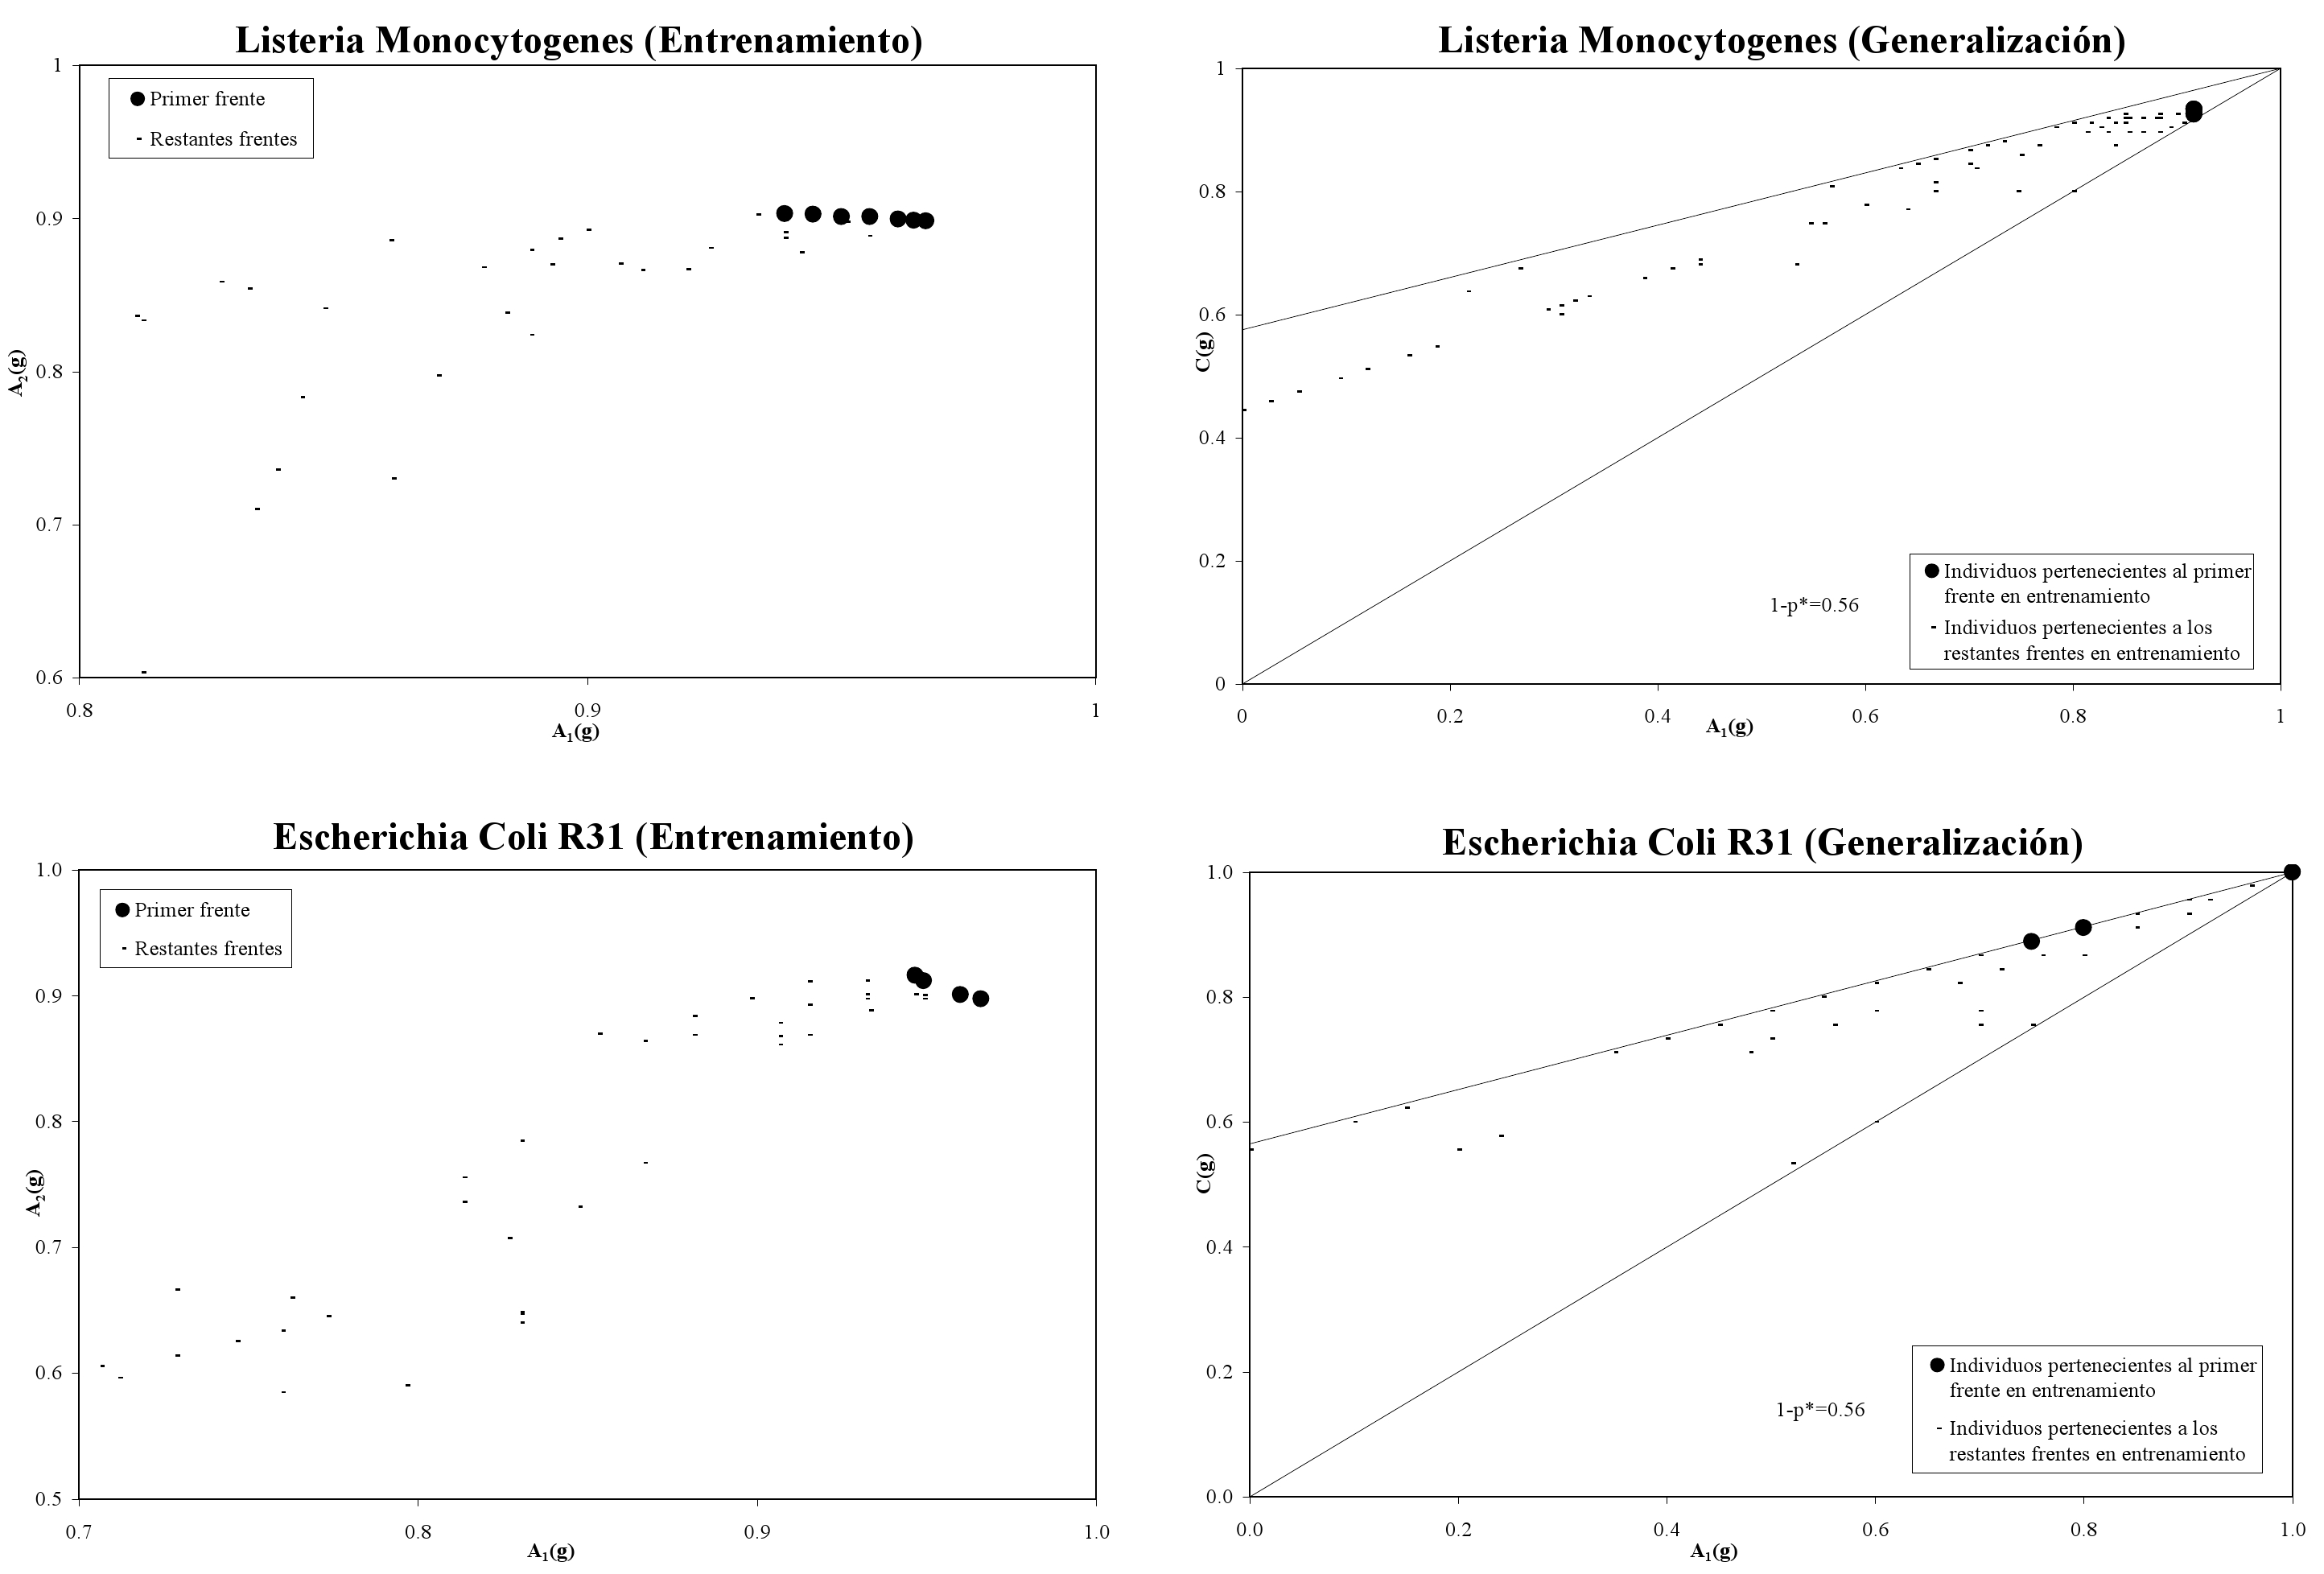
\includegraphics[keepaspectratio,width=17cm]{figuras/frentes_ASC09_tanda1.jpg}
		\caption{Frente de Pareto en entrenamiento en el plano $(A_{1},A_{2})$ y
				valores en generalización en el plano $(MS,C)$ para \textit{L. Monocytogenes},
\textit{E. Coli R31} en una ejecución específica.}
	\label{fig1frentes}
\end{figure}
\end{landscape}

\begin{landscape}
\begin{figure}[!htb]
\centering
	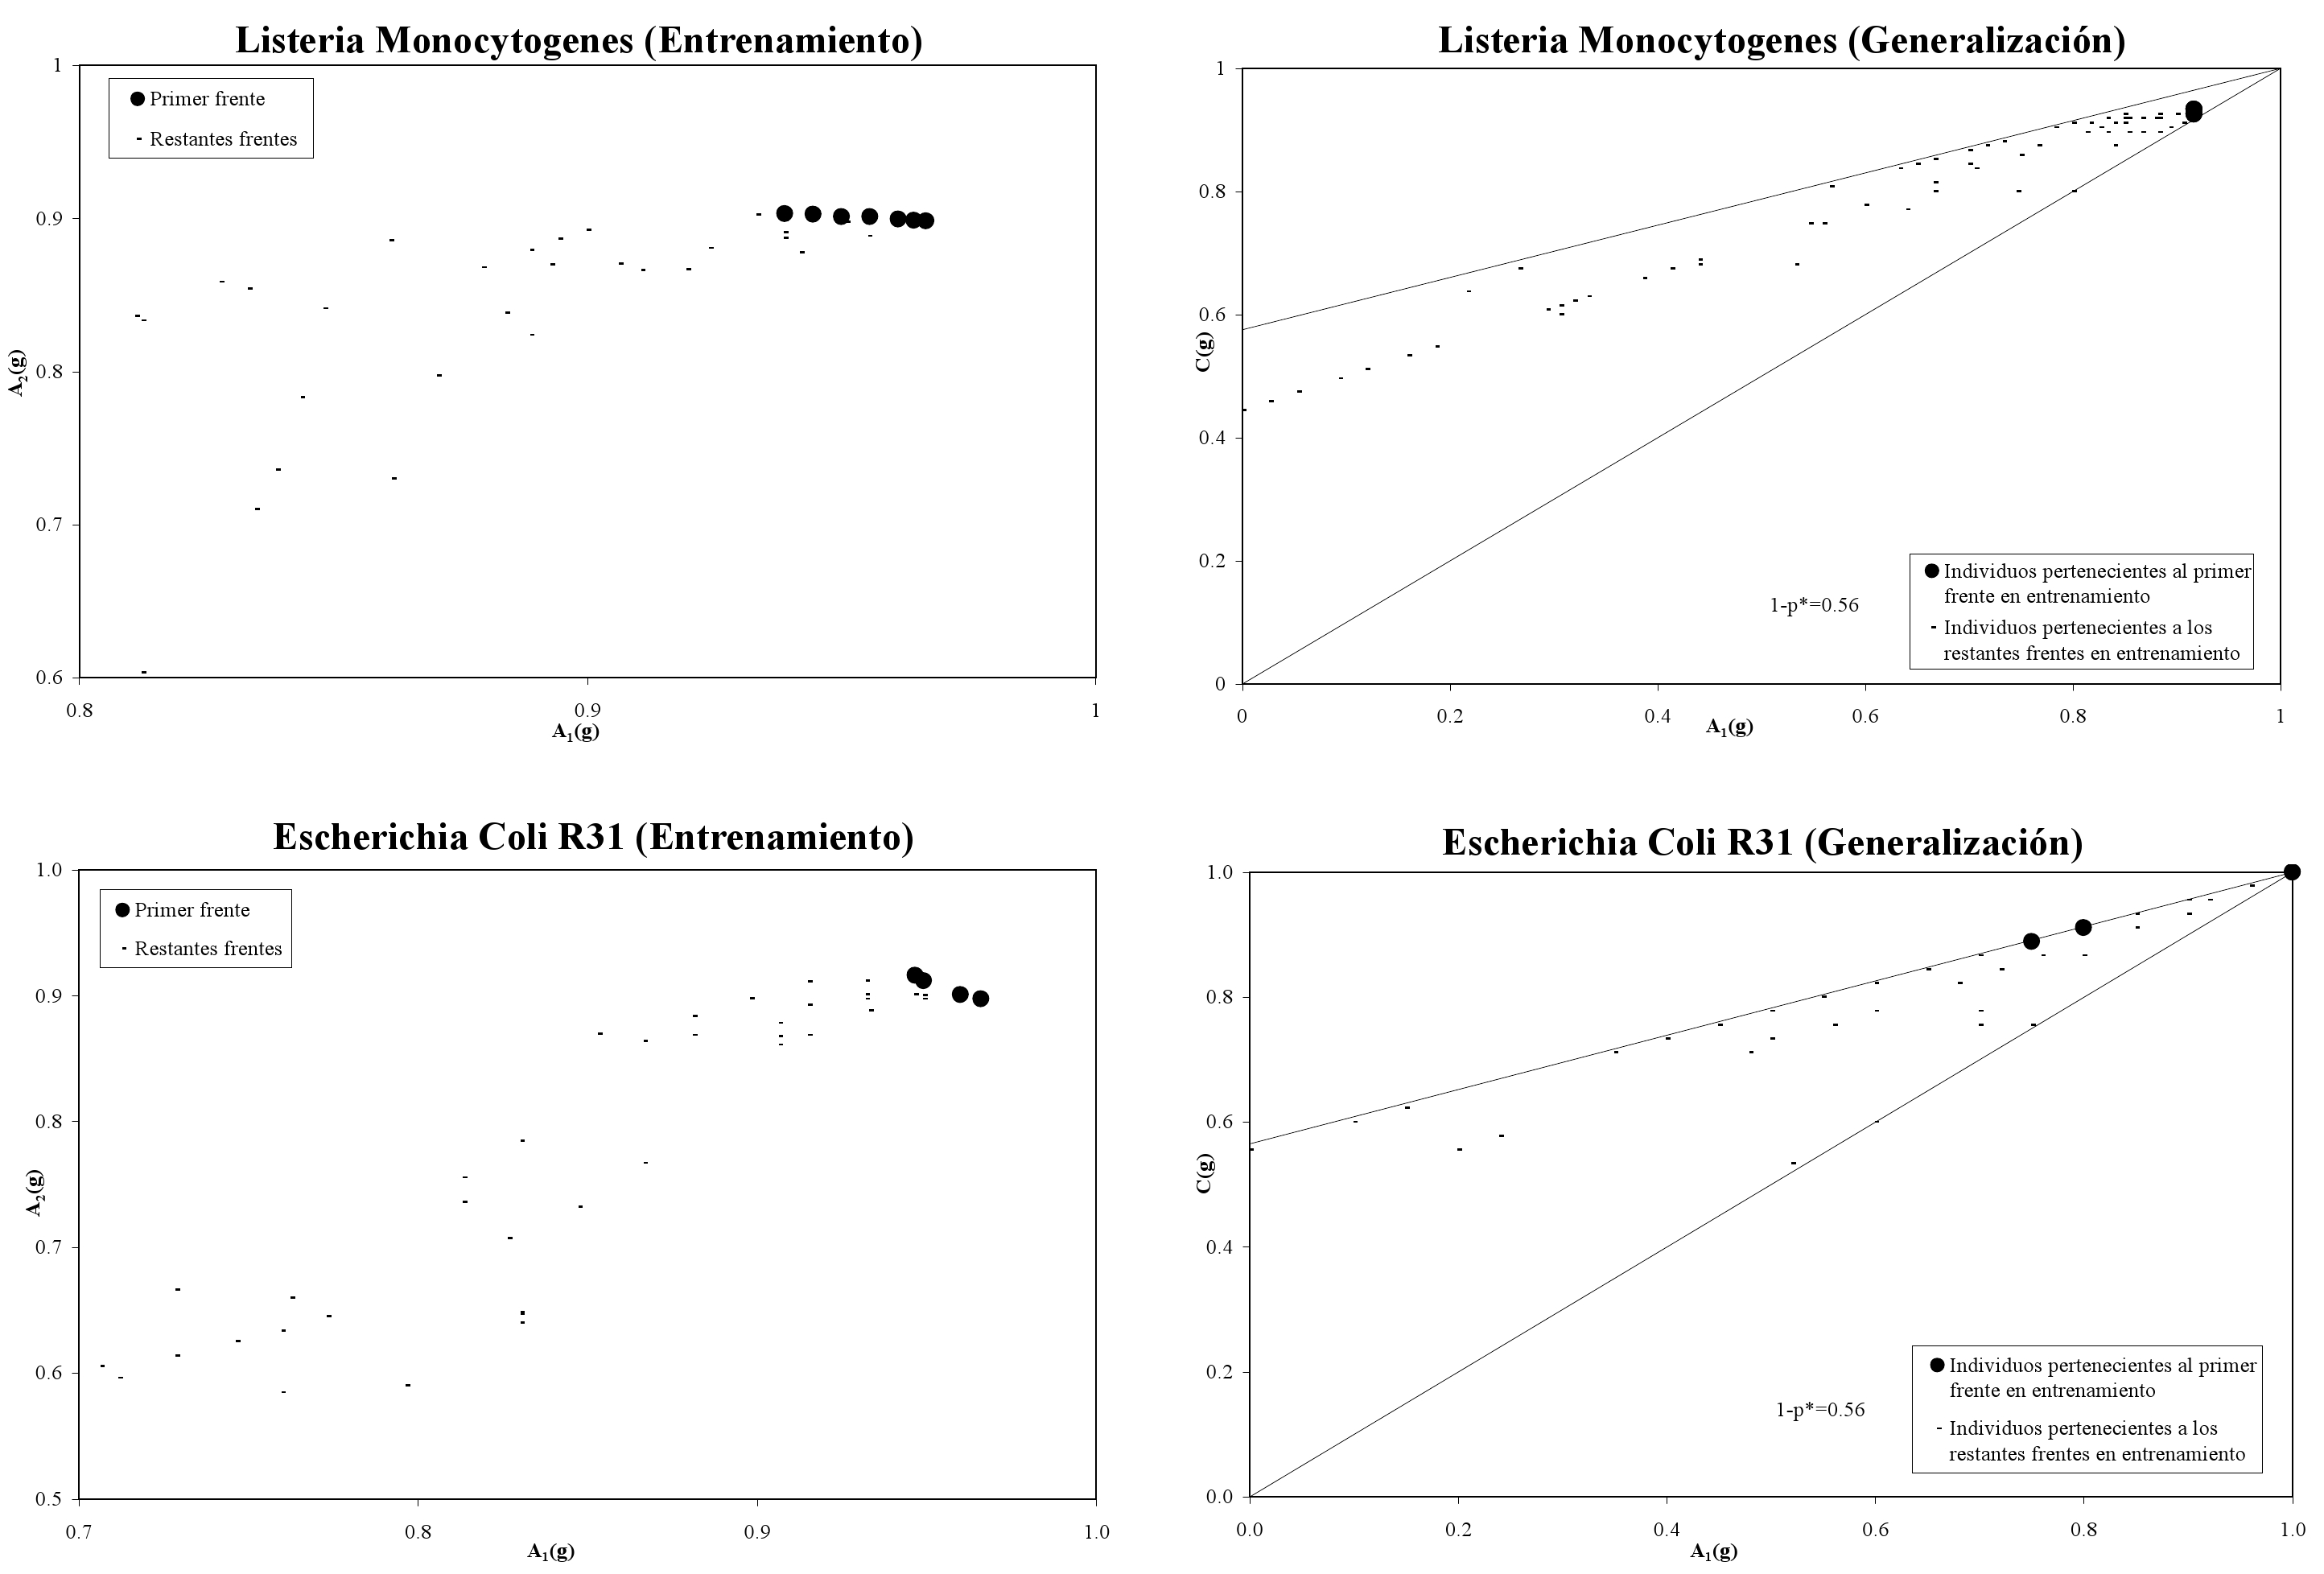
\includegraphics[keepaspectratio,width=17cm]{figuras/frentes_ASC09_tanda1.jpg}
		\caption{Frente de Pareto en entrenamiento en el plano $(A_{1},A_{2})$ y
valores en generalización en el plano $(MS,C)$ para \textit{S. Aureus} y \textit{S.
Flexneri} en una ejecución específica.}
	\label{fig2frentes}
\end{figure}
\end{landscape}

Los valores extremos $(+)$, son datos de
las métricas por encima de los extremos de las dos barras. Para los algoritmos
deterministas sólo tenemos un resultado para cada patógeno, por lo tanto los
valores del cuartil inferior y superior, y la observación más pequeña y más grande, no se
puede representar. Como podemos ver en las figuras \ref{fig1aplica} a la \ref{fig4aplica}, en $C$,
el
grado de dispersión de M-E y R-F es menor que el grado de dispersión de los resultados generados por
M-S. En $MS$, el grado de dispersión de M-E es, en general, inferior a R-F y M-S. En $RMSE$ el
grado de dispersión es bajo y muy similar para las tres metodologías. En $AUC$, el grado de
dispersión también es bajo y similar en todas las metodologías.

Finalmente, cabe destacar que los modelos evolutivos obtenidos mediante MPENSGAII proporcionan
redes MLP con valores crecientes de $E$ y $MS$ en el comienzo de la evolución. Cuando se
alcanzan valores altos de $E$ y/o $MS$ sobre el conjunto de entrenamiento, las metodologías
MPENSGAII obtienen frentes de Pareto con modelos que tienen una precisión alta sin reducir el nivel
de $MS$ y viceversa. Por otra parte, cabe señalar que los valores de $MS$ obtenidos por la
metodología M-E son similares, o incluso mejores, que los valores obtenidos con otras metodologías
bien
conocidas en \textit{Machine Learning}, y que se obtiene una mayor precisión de clasificación en
generalización para las dos clases de cada patógeno. Por otra parte, la metodología M-S también da
lugar a valores muy altos de $C$ y $MS$.

Los resultados estadísticos obtenidos y los test de comparaciones múltiples analizados muestran que
M-E es un método competitivo en microbiología predictiva, donde hay
una
necesidad alta de obtener una buena precisión en la clasificación, tanto para el crecimiento como
para el no
crecimiento. Este enfoque puede ayudar a los investigadores en microbiología predictiva
a definir mejor los límites de crecimiento de los microorganismos, y también para modelar la
variabilidad microbiana asociada a las condiciones ambientales. En conclusión, la utilización de
este método
constituye una alternativa valiosa para la creación de modelos matemáticos que determinen la
probabilidad de crecimiento microbiano bajo un determinado conjunto de condiciones.

\begin{landscape}
\begin{figure}[!htb]
\centering
	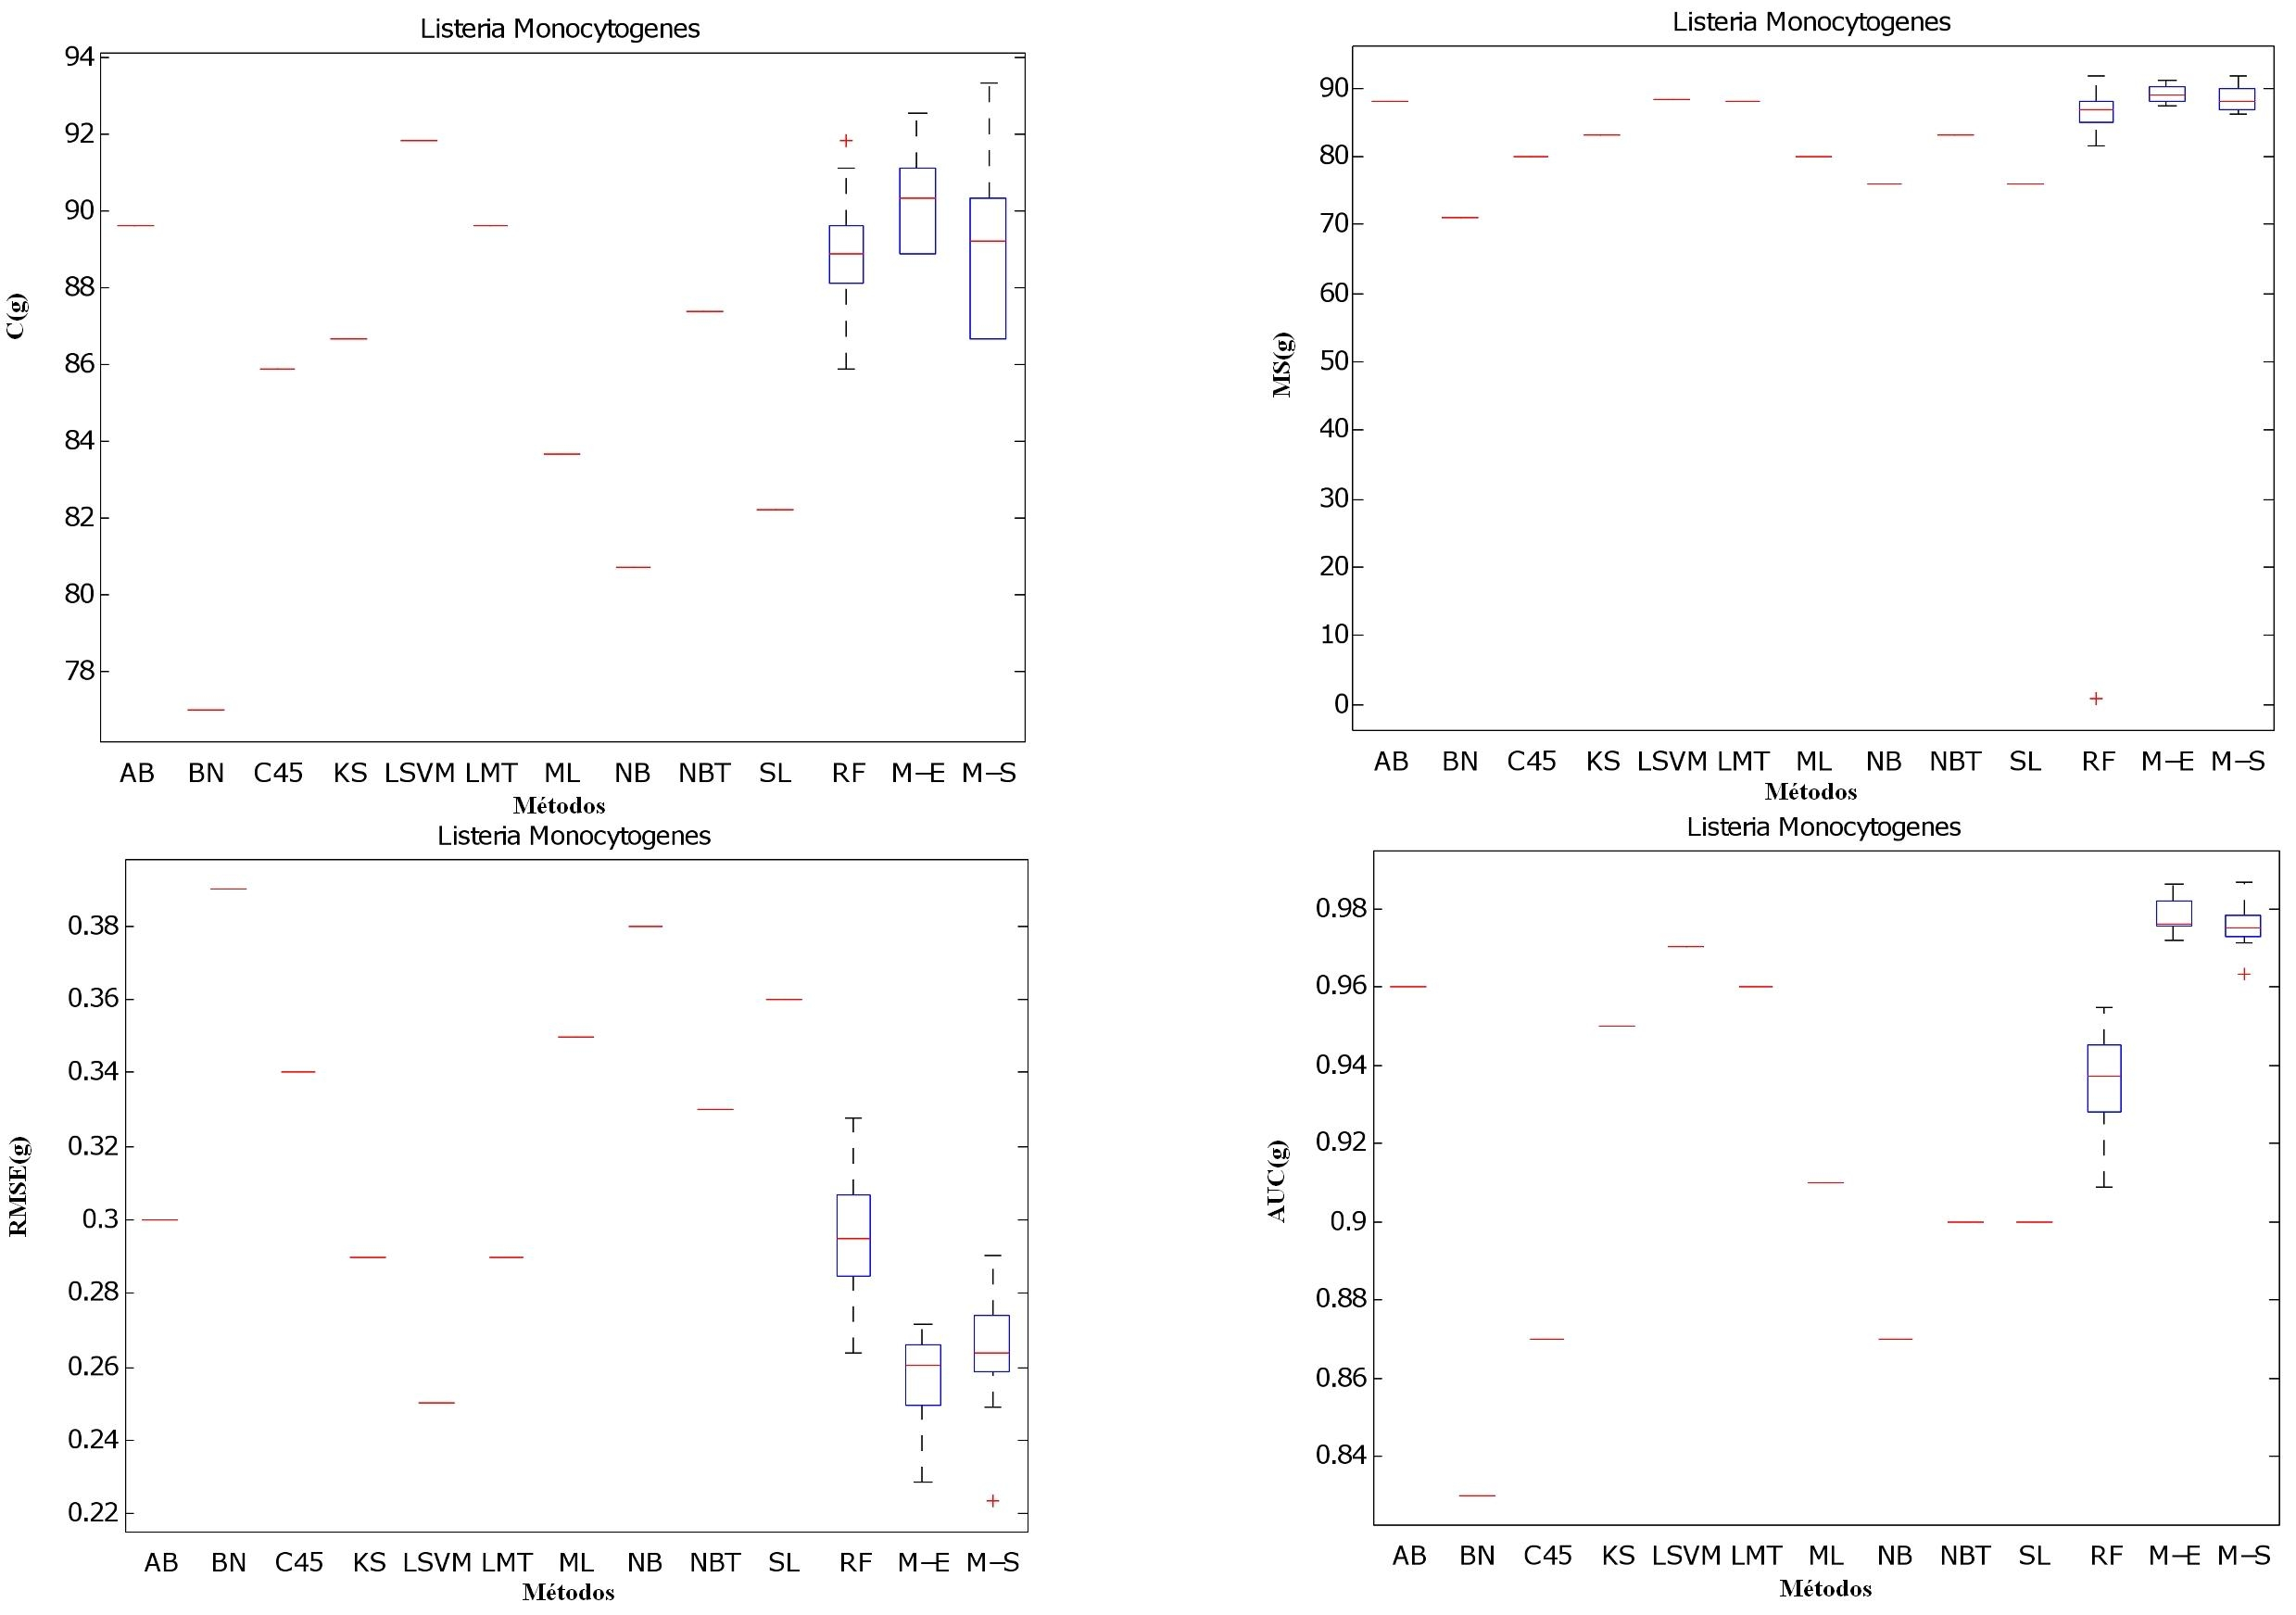
\includegraphics[keepaspectratio,width=17cm]{figuras/BoxPlot_tanda1.jpg}
	\caption{Métricas $C$, $MS$, $RMSE$ y $AUC$ en los diagramas de cajas para
\textit{L. Monocytogenes}.}
	\label{fig1aplica}
\end{figure}
\end{landscape}

\begin{landscape}
\begin{figure}[!htb]
\centering
	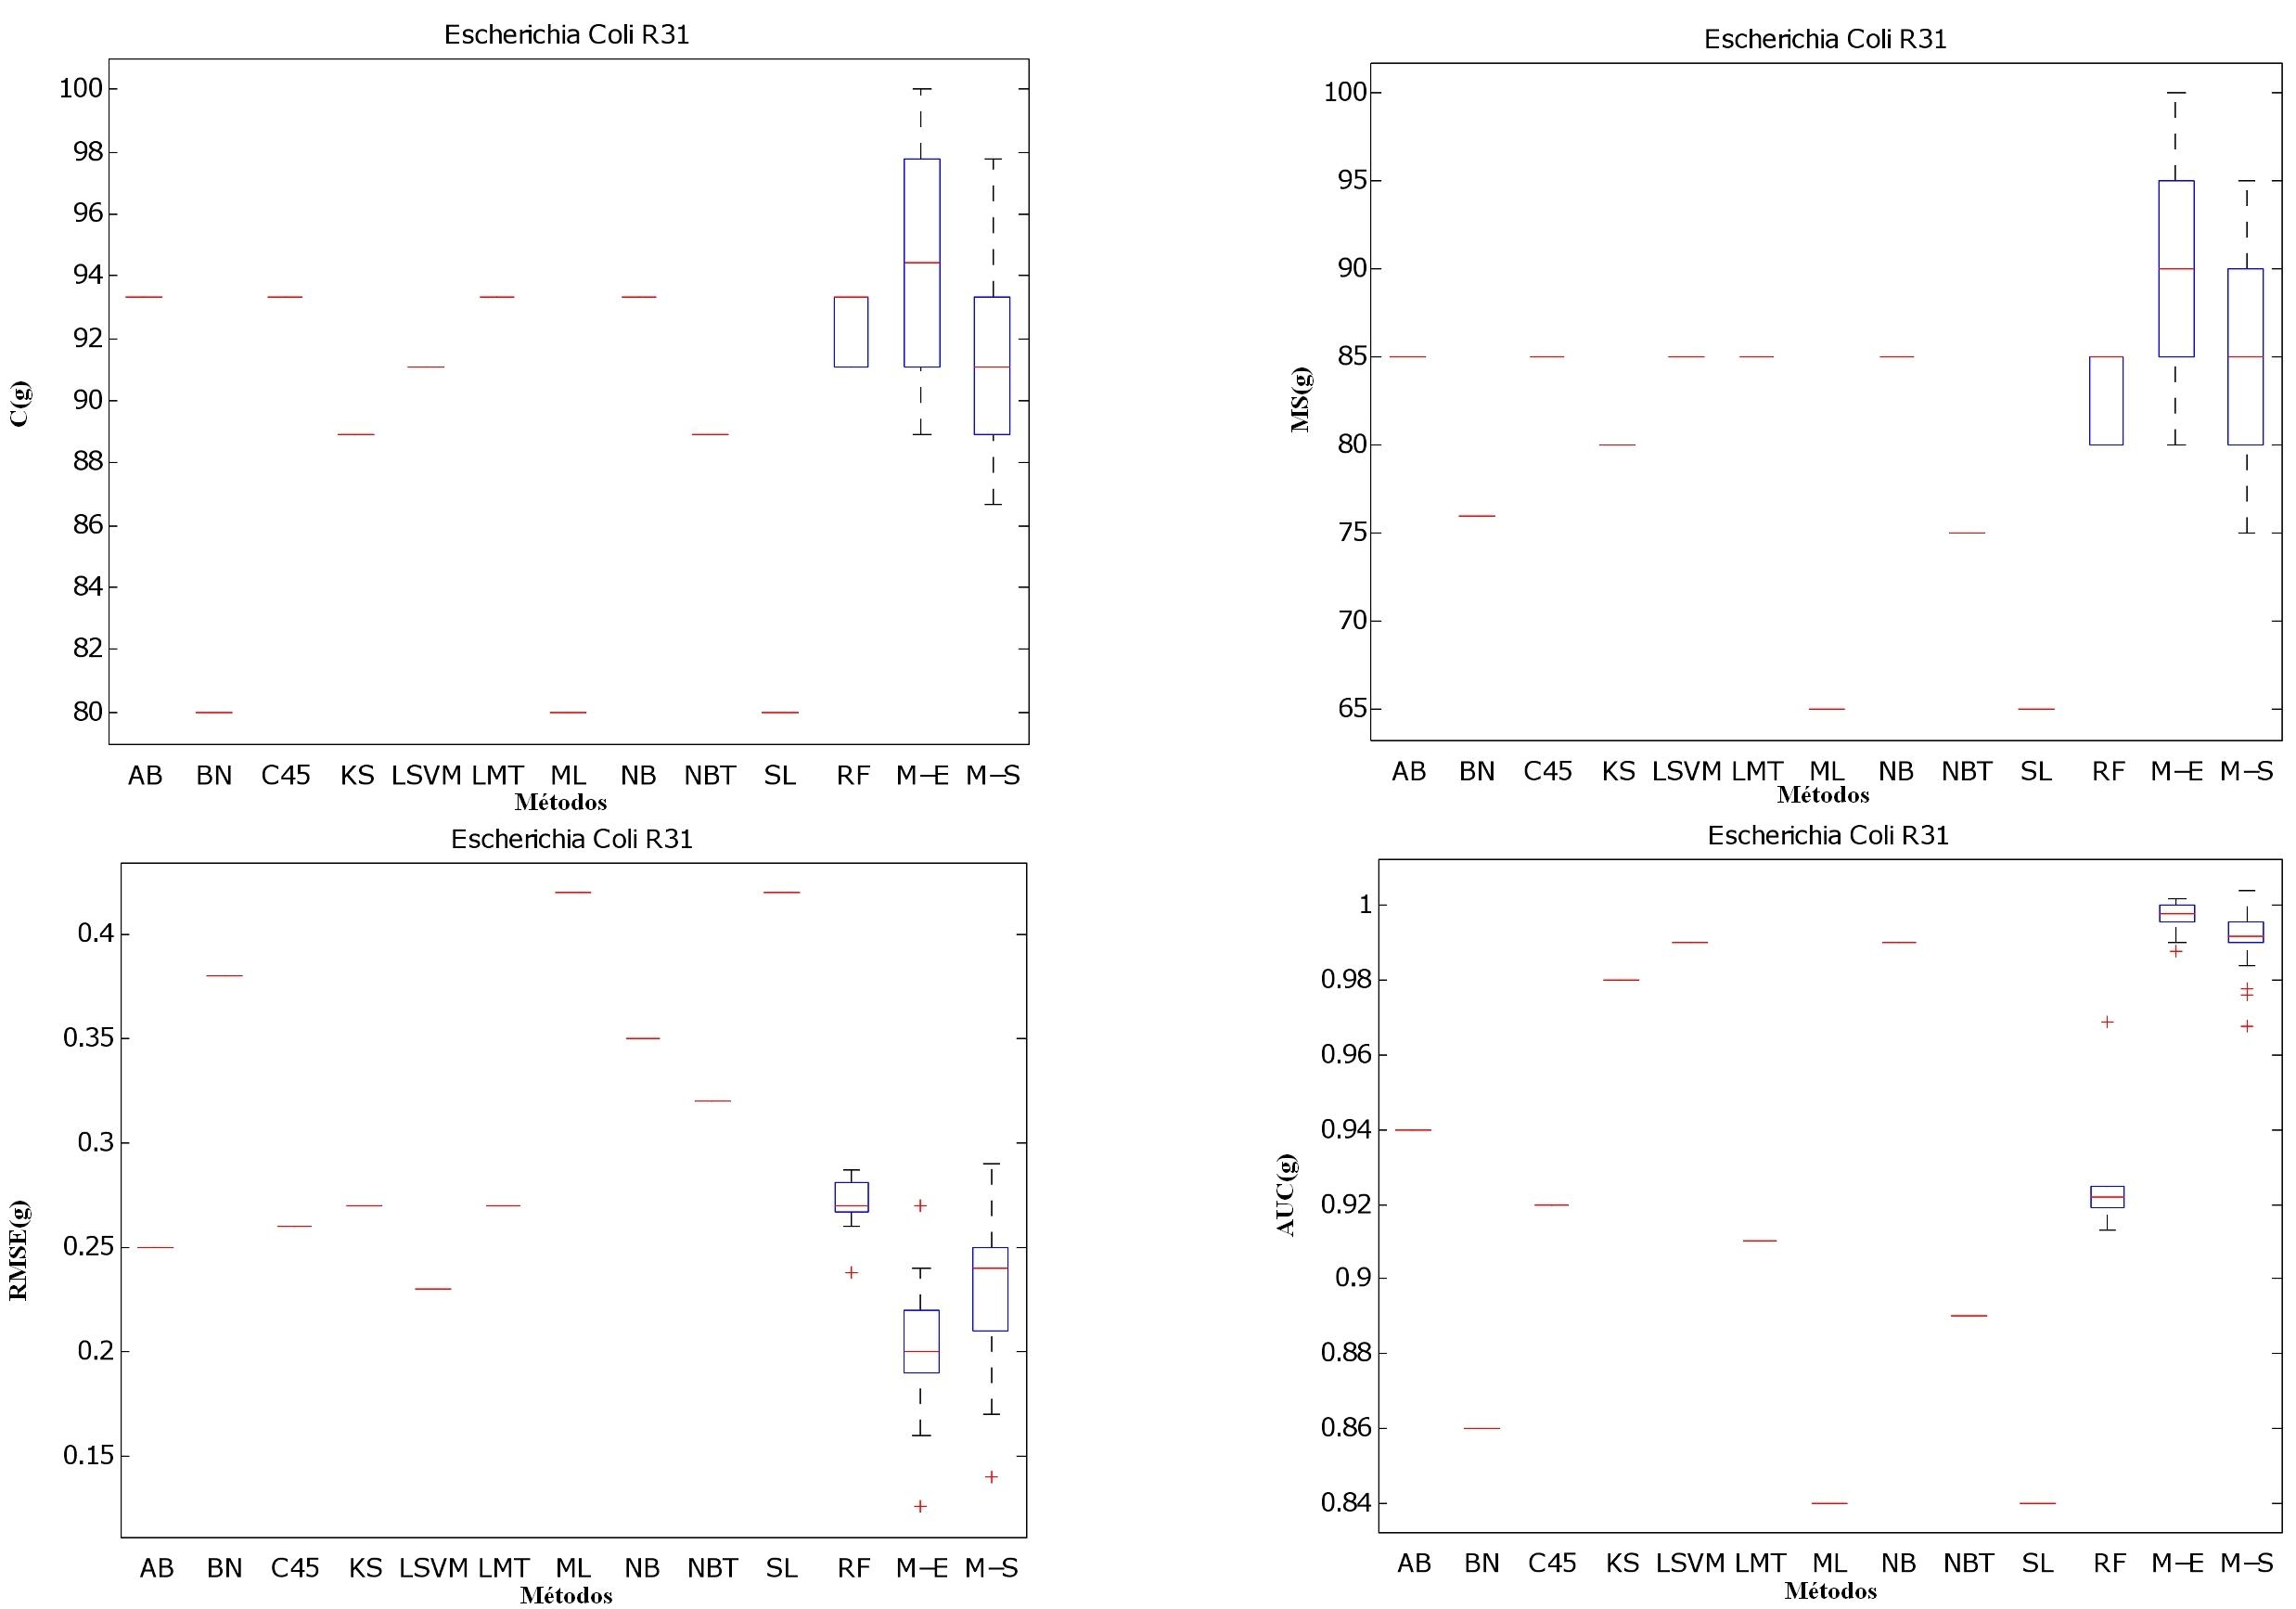
\includegraphics[keepaspectratio,width=17cm]{figuras/BoxPlot_tanda2.jpg}
\caption{Métricas $C$, $MS$, $RMSE$ y $AUC$ en los diagramas de cajas para
\textit{E. Coli R31}.}
\label{fig2aplica}
\end{figure}
\end{landscape}

\begin{landscape}
\begin{figure}[!htb]
\centering
	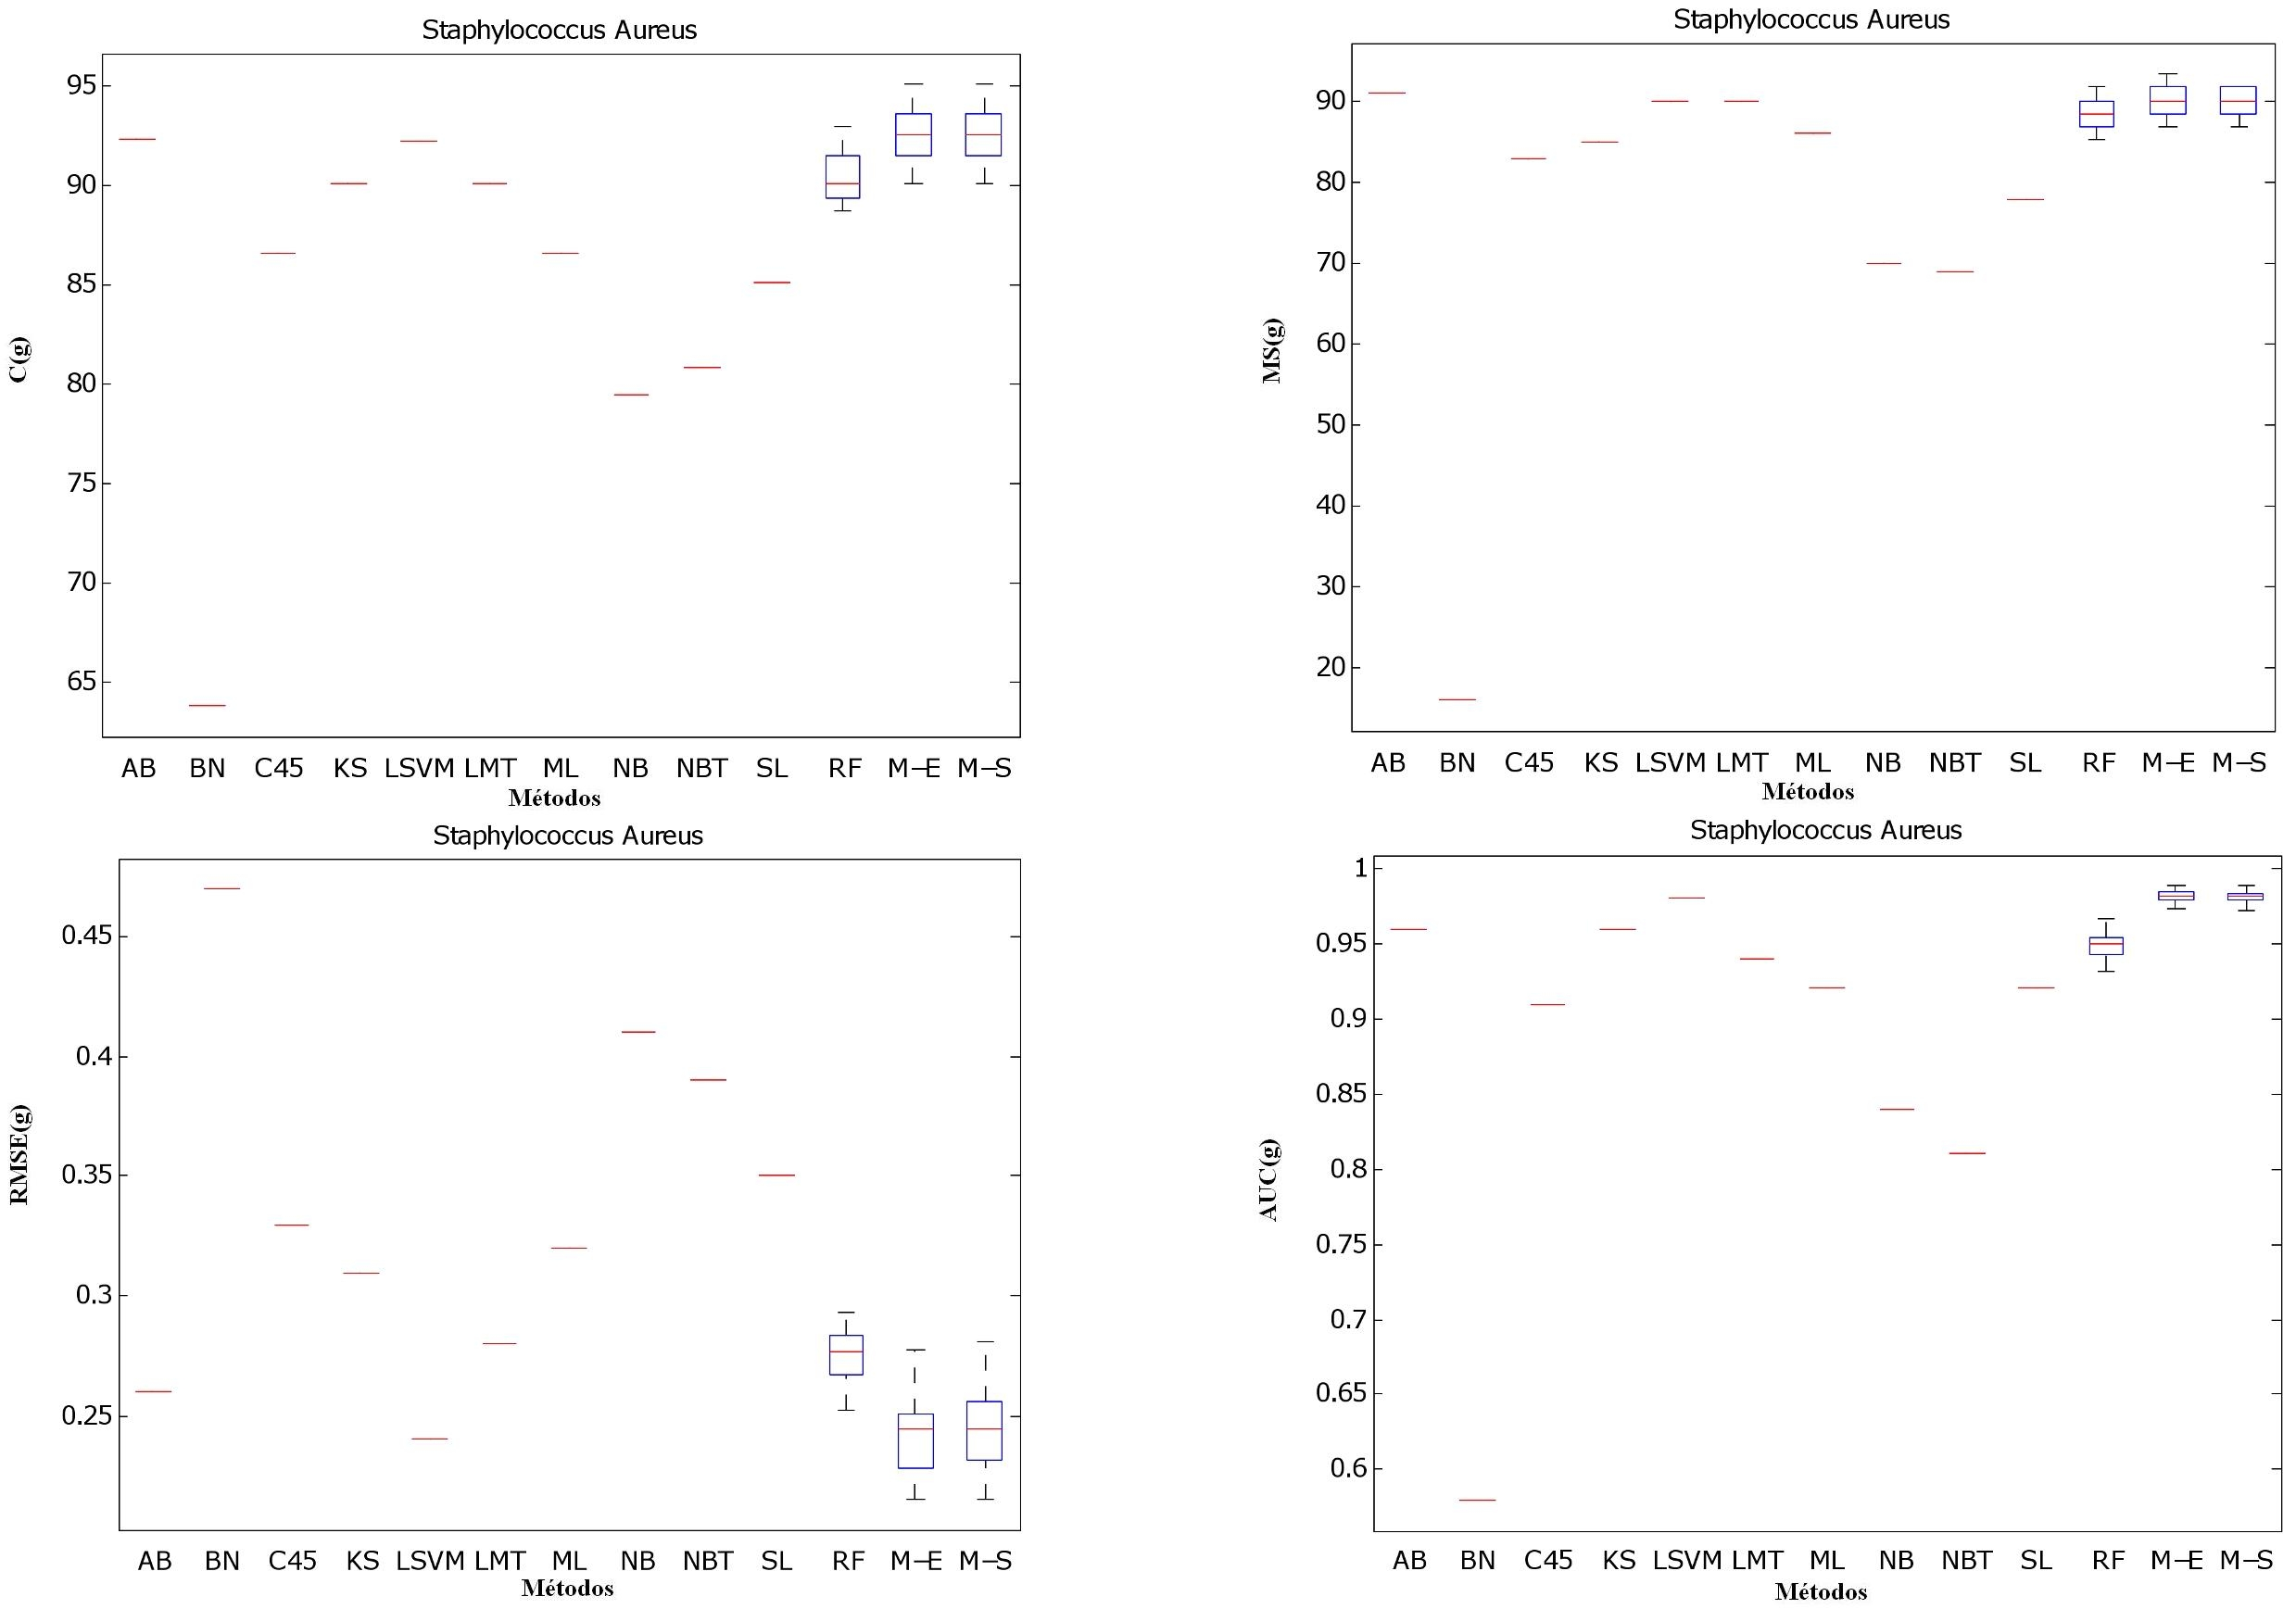
\includegraphics[keepaspectratio,width=17cm]{figuras/BoxPlot_tanda3.jpg}
		\caption{Métricas $C$, $MS$, $RMSE$ y $AUC$ en los diagramas de cajas para
		\textit{S. Aureus}.}
\label{fig3aplica}
\end{figure}
\end{landscape}

\begin{landscape}
\begin{figure}[!htb]
\centering
	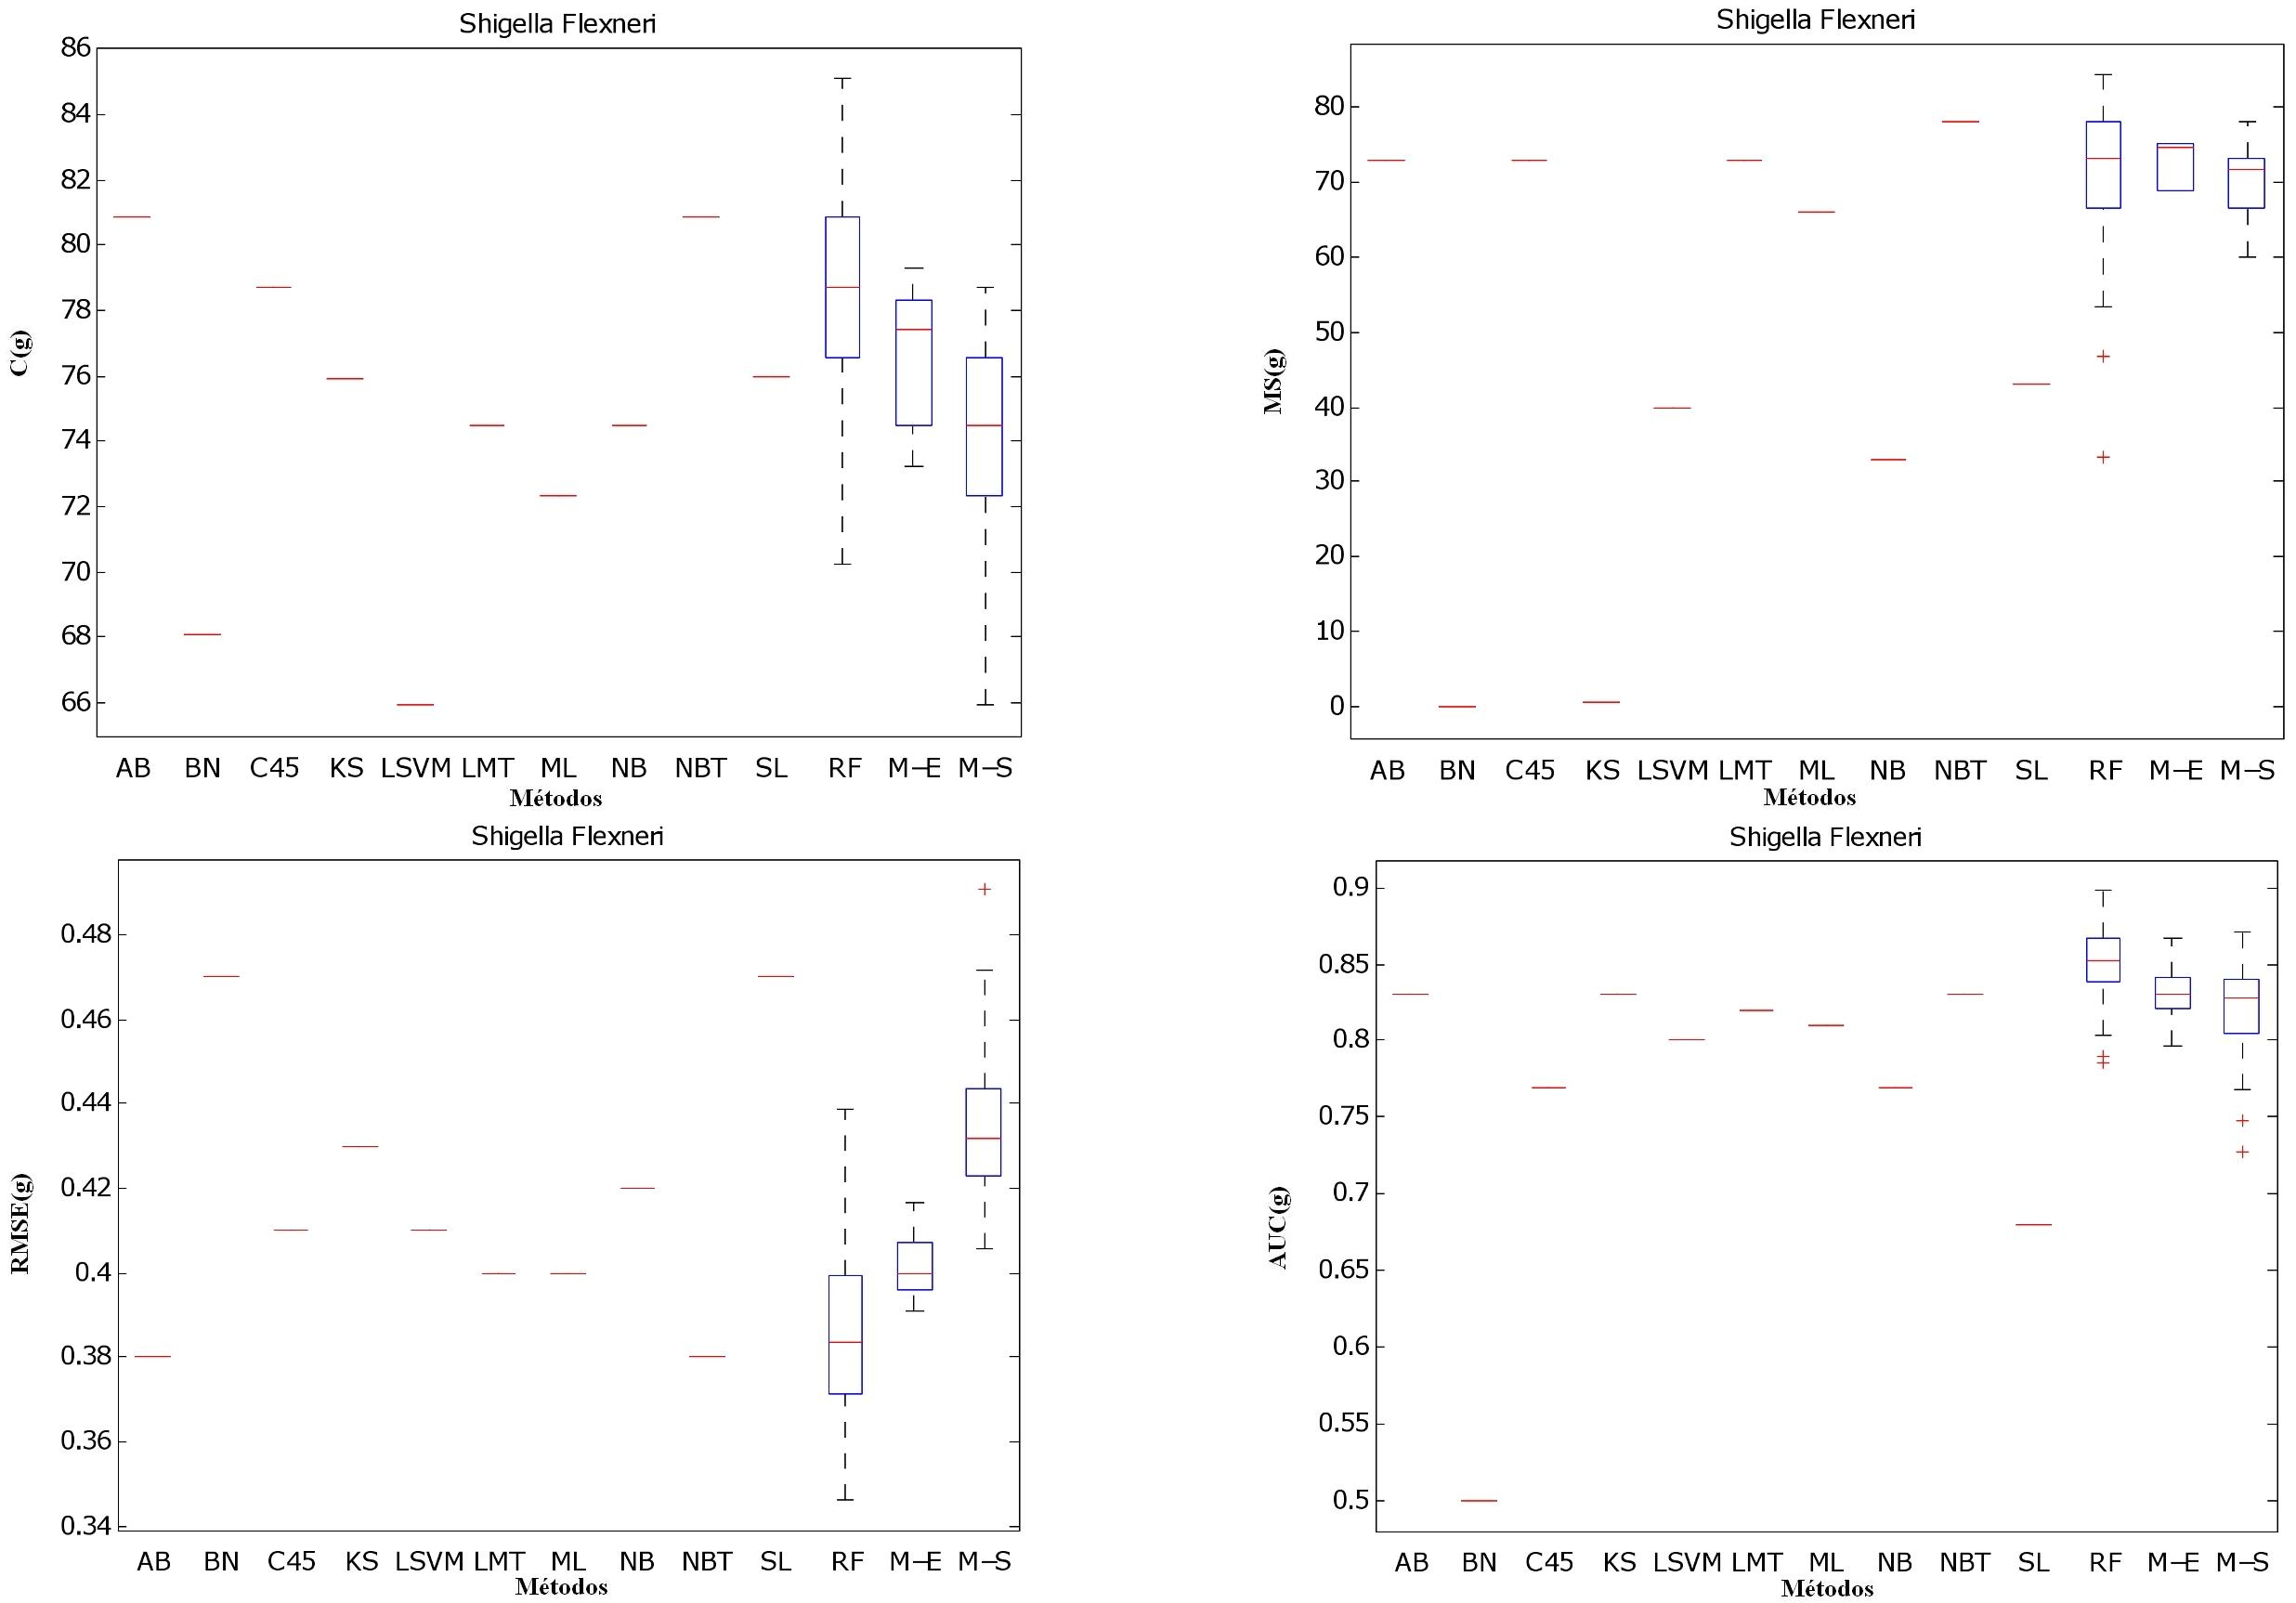
\includegraphics[keepaspectratio,width=17cm]{figuras/BoxPlot_tanda4.jpg}
	\caption{Métricas $C$, $MS$, $RMSE$ y $AUC$ en los diagramas de cajas para
\textit{L. Flexneri}.}
	\label{fig4aplica}
\end{figure}
\end{landscape}
% \paginavaciasincuerpo
